\documentclass{cmspaper}
\usepackage{graphicx}
\usepackage{rotate}
\usepackage{relsize}
\usepackage{lineno}

\newcommand{\met} {\ensuremath{E\!\!\!\!/_T}}
\newcommand{\ttbar} {\ensuremath{t\bar{t}~}}
\newcommand{\ptll} {\ensuremath{P_T(\ell\ell)}}
\newcommand{\ptllres} {\ensuremath{P^{\rm res}_T(\ell\ell)}}
\def\ack{\section*{Acknowledgments}}

\linenumbers

\begin{document}

%==============================================================================
% title page for many authors
%
\begin{titlepage}
\title{Search for New Physics in the Same Sign Dilepton final state with b Jets and Missing Energy at the LHC}

  \begin{Authlist}
    D.~ Barge, C.~Campagnari, P.~Kalavase, D.~Kovalskyi, V.~Krutelyov, J.~Ribnik
    \Instfoot{ucsb}{University of California, Santa Barbara}
    W.~Andrews, G.~Cerati, D.~Evans, F.~Golf, I.~MacNeill, S.~Padhi, Y.~Tu, F.~W\"urthwein, A.~Yagil, J.~Yoo
    \Instfoot{ucsd}{University of California, San Diego}
    L.~Bauerdick, I.~Bloch, K.~Burkett, I.~Fisk, Y.~Gao, O.~Gutsche, B.~Hooberman, S.~Jindariani, J.~Linacre
    \Instfoot{fnal}{Fermi National Accelerator Laboratory, Batavia, Illinois}
  \end{Authlist}

\begin{abstract}
We search for New Physics in the same sign dilepton final state with at least two b jets 
and \met~. The search is performed in a data sample collected with the CMS detector
of pp collisions at a centre-of-mass energy of 7 TeV, corresponding to an integrated
luminosity of $349$ pb$^{-1}$. For these searches, the dominant background is from \ttbar 
events. No excess above the standard model background expectation is observed.
Upper limits at 95\% confidence level are set on the number of observed events.
%pMSSM as well as the simplified models 
%involving stop and sbottom productions.
\end{abstract}
\end{titlepage}

\section{Introduction}
\label{sec:intro}

After the successful operation of the Large Hadron Collider (LHC) and the CMS detector
in 2010 and 2011, and with good prospects for the future, the LHC is now ready to shed light on a number 
of open questions in Particle Physics 
such as the mechanism of electroweak (EW) symmetry breaking, or the 
new physics, Beyond the Standard Model (BSM), that stabilizes the EW scale. 

A wealth of theories that extend the Standard Model have been put forth during the past decades. Supersymmetry (SUSY) is
arguably the best motivated BSM theory --- and certainly the most 
thoroughly studied. 
Indeed, searches for SUSY are among the primary objectives of the 
CMS experiment. SUSY is exceedingly popular not 
only for its theoretical beauty but also because SUSY phenomenology 
is extremely rich, 
%in fact is can mimic almost any other new physics scenario. 
leading to a large variety of possible new signals at the LHC. 
In spite of this, the majority of SUSY studies focus on a very special 
setup: the so-called Constrained Minimal Supersymmetric Standard Model (CMSSM). 
This was justified in the preparation for discoveries as the CMSSM, 
having just a handful of new parameters, is very predicive. However, 
the simplifying assumption of universality at the GUT scale lacks a sound 
theoretical motivation. Consequently, the CMSSM should be regarded as a showcase 
model. When it comes to interpreting experimental results, it is reasonable and interesting to do this within the CMSSM because it 
provides (to some degree) an easy way to show performances, 
compare limits or reaches, etc. However, the interpretation of experimental results in the 
$(m_0,m_{1/2})$ plane risks imposing unwarranted constraints on SUSY, as many 
mass patterns and signatures that are possible a priori are not covered in the CMSSM. 
The same problem arises in any analysis that assumes a particular 
SUSY breaking scheme. 

In this document, we therefore introduce a different approach, which uses only 
minimal assumptions on the underlying SUSY parameters. In particular, given the absence of experimental guidance, we choose
not to rely on a particular SUSY breaking scheme.
Instead, we use a 19-dimensional 
parametrization of the MSSM, called the \emph{phenomenological MSSM} (pMSSM),
with parameters defined not at the GUT scale but instead at the SUSY scale 
(by convention the geometric mean of the two stop masses).
We demonstrate the feasibility of our approach by applying it to 
the 2011 CMS data-set corresponding to 1~fb$^{-1}$ of integrated luminosity.  
Using profile likelihoods, we combine 
the dijet $\alpha_T$ analysis, the opposite-sign dilepton 
analysis and the same-sign dilepton analysis and derive constraints 
on the SUSY particles with as few simplifying assumptions as possible.
Results from other SUSY analyses in CMS will be added as soon as they become available.

We first give the motivation to go beyond the CMSSM and work in 
a generic MSSM setup. After this, the pMSSM and its parametrization is defined. 
We then outline our analysis, giving details on the pMSSM points we have used, 
the detector simulation and the CMS analyses, and describe the statistical method based on 
profile likelihoods used for coping with the 19-dimensional model. Finally, we discuss our results and summarize our conclusions.


%\section{Simulated Event samples}
\label{sec:mcsignal}

In the MSSM, the scalar partners of the left- and right-handed squarks, $\tilde{q_L}$
and $\tilde{q_R}$, can mix to form mass eigenstates. These mixing effects thus leads to different fermion
masses and therefore becomes important for the third generation. The large mixing can yield sbottom ($\tilde{b_1}$)
and stop ($\tilde{t_1}$) eigenstates which are significantly lighter than other squarks. This also implies  $\tilde{b_1}$
and $\tilde{t_1}$ could be produced with larger cross sections then the light flavour squarks at the LHC. Consequently, 
the subsequent decays of $\tilde{b_1}$ and $\tilde{t_1}$ can lead to same sign dileptons in association with b quarks.
Furthermore, the $\tilde{g}\tilde{g}$ productions via $\tilde{\chi}^\pm_1$ such as $\tilde{g} \rightarrow \tilde{\chi}^{+}_{1} b \bar{t}$
can also give rise to same sign dileptons with b jets.

\section{Search for same-sign dileptons with $b$ jets}
\label{sec:searchbtag}

This analysis is based on the same-sign dilepton search documented in AN-2011/258~\cite{ssnote2011} and corresponds to an
integrated luminosity of \intLumi. In that study we searched for events with two isolated same-sign leptons
in association with 2 additional jets and \met. Here we re-use most of the baseline event selection~\footnote{The additional 
$Z$ veto is not applied in this study} as summarized in Section~\ref{sec:eventsel} below. 
In addition, we require at least 2 b-tagged jets using Track Counting High Efficiency 
Medium (TCHEM) working point tagger~\cite{BTVPAS2011}. We refer to TCHEM with the requirement that three of the tracks have $IP$ 
significance $ > 3.3$. For this tagger the expected b-tagging efficiency is 62\% with a roughly 20\% systematic uncertainty.
The acceptance of light flavor jets is $\sim 2$\%~\cite{BTVPAS2011}.

\subsection{Event Selection}
\label{sec:eventsel}

As mentioned previously, this search is a refinement of~\cite{ssnote2011}, and we thus discuss here only differences and briefly summarize the basic kinematics and triggers.
For more details, we refer to~\cite{ssnote2011}.

\begin{itemize}
\item At least two isolated same-sign leptons ($ee$, $e\mu$, and $\mu\mu$) with $|\eta| < 2.4$.
\item We require both leptons to have $p_T>$20 GeV.
\item We tighten the isolation cut on the leptons to 0.1.
\item At least two particle flow jets tagged using SSVHEM tagger with $p_T > 40$ GeV and $|\eta| < 2.4$
%{\it why not 3.0 ??} 
corrected with L1FastL2L3 corrections.
\item The selected jets must be separated from the leptons by $\Delta R > 0.4$.
\item \met $> 30$ GeV.
\item We remove dilepton events with invariant mass $M_{ll} < 8$ GeV.
%{\it switched to tighter mll cut because we can.}
\end{itemize}

More details are found in Reference~\cite{ssnote2011}.

\subsection{Event Yields and Background Estimation}
\label{eventsel}

The results of this search in the above-mentioned kinematical region are summerized in Table~\ref{tab:ssyields1}.
As mentioned in the introduction, and quantified by this table, SM background is expected to be dominated by $t\bar{t}$ production
with one real and one fake lepton.
We estimate this background from the data itself using the ``Tight-To-Loose ratio'' (Fake Rate) method~\cite{frmethod}.
Electron charge mis-reconstruction is estimated by weighting opposite-sign dilepton events that pass all our cuts
by a charge flip rate obtained form single electron Monte Carlo as described in detail in~\cite{ssnote2011}.
The probability for muons to be reconstructed with the wrong sign in the relevant momemtum range is negligible.
Both of these techniques are described in more detail in~\cite{ssnote2011}.
Systematic errors on these two estimates are 50\% and 25\% respectively.

In addition, we use MC to estimate contributions from the following additional SM production processes.
All of these are quite small.

\begin{itemize}
\item $qqW^\pm W^\pm, WWW, t\bar{t}W$, and double parton $W^\pm W^\pm$ with two real leptons in the final state.
\item $WZ$ and $ZZ$ with two real leptons in the final state.
\item $W\gamma$ with one real lepton and a photon conversion. This background is a priori not estimated by the fake rate method
because the photon is generally isolated. In practice, this background is completely negligible.
\end{itemize}

{\it Need to update the tables to include the remaining MC bkg as the MC becomes available !!!}

\newcommand{\ttdilS}{\ensuremath{\ttbar\to\ell\ell X}}
\newcommand{\ttslbS}{\ensuremath{\ttbar\to\ell(b\to\ell) X}}
\newcommand{\ttsloS}{\ensuremath{\ttbar\to\ell(b\!\!\!/\to\ell) X}}
\newcommand{\SFnn}{\ensuremath{N^{\rm Wj,raw}_{nn}}}

\begin{table}[h]
\begin{center}
\begin{tabular}{l | l l l l}
\hline\hline
 Source  &  ee  &  $\mu\mu$  &  e$\mu$  &  all \\
\hline
$t\overline{t}\rightarrow \ell\ell X$ &  0.469 $\pm$  0.305 &  0.000 $\pm$  0.199 &  1.133 $\pm$  0.580 &  1.603 $\pm$  0.656\\
$t\overline{t}$ other &  0.000 $\pm$  0.199 &  0.000 $\pm$  0.199 &  0.000 $\pm$  0.199 &  0.000 $\pm$  0.199\\
$t\overline{t}\rightarrow \ell(b\rightarrow \ell)X$ &  0.000 $\pm$  0.199 &  0.193 $\pm$  0.143 &  0.000 $\pm$  0.199 &  0.193 $\pm$  0.143\\
$t\overline{t}\rightarrow \ell(\slashed{b}\rightarrow \ell)X$ &  0.563 $\pm$  0.399 &  0.000 $\pm$  0.199 &  0.143 $\pm$  0.131 &  0.706 $\pm$  0.420\\
\hline
$t$, s-channel &  0.000 $\pm$  0.057 &  0.000 $\pm$  0.057 &  0.000 $\pm$  0.057 &  0.000 $\pm$  0.057\\
$t$, t-channel &  0.077 $\pm$  0.077 &  0.000 $\pm$  0.055 &  0.000 $\pm$  0.055 &  0.077 $\pm$  0.077\\
$tW$ &  0.000 $\pm$  0.045 &  0.000 $\pm$  0.045 &  0.016 $\pm$  0.045 &  0.016 $\pm$  0.045\\
\hline
$Z\rightarrow ee$ &  0.000 $\pm$  0.429 &  0.000 $\pm$  0.429 &  0.000 $\pm$  0.429 &  0.000 $\pm$  0.429\\
$Z\rightarrow\mu\mu$ &  0.000 $\pm$  0.429 &  0.000 $\pm$  0.429 &  0.000 $\pm$  0.429 &  0.000 $\pm$  0.429\\
$Z\rightarrow\tau\tau$ &  0.000 $\pm$  0.429 &  0.000 $\pm$  0.429 &  0.000 $\pm$  0.429 &  0.000 $\pm$  0.429\\
$W$+jets &  0.000 $\pm$  1.808 &  0.000 $\pm$  1.808 &  0.000 $\pm$  1.808 &  0.000 $\pm$  1.808\\
$WW$ &  0.000 $\pm$  0.019 &  0.000 $\pm$  0.019 &  0.000 $\pm$  0.019 &  0.000 $\pm$  0.019\\
\hline
V$\gamma$ &  0.000 $\pm$  0.248 &  0.000 $\pm$  0.248 &  0.000 $\pm$  0.248 &  0.000 $\pm$  0.248\\
$W\gamma^{*}\rightarrow\ell\nu e e$ &  0.000 $\pm$  0.097 &  0.000 $\pm$  0.097 &  0.000 $\pm$  0.097 &  0.000 $\pm$  0.097\\
$W\gamma^{*}\rightarrow\ell\nu\mu\mu$ &  0.000 $\pm$  0.075 &  0.000 $\pm$  0.075 &  0.000 $\pm$  0.075 &  0.000 $\pm$  0.075\\
$W\gamma^{*}\rightarrow\ell\nu\tau\tau$ &  0.000 $\pm$  0.028 &  0.000 $\pm$  0.028 &  0.000 $\pm$  0.028 &  0.000 $\pm$  0.028\\
$WZ$ &  0.034 $\pm$  0.012 &  0.017 $\pm$  0.008 &  0.031 $\pm$  0.012 &  0.082 $\pm$  0.019\\
$ZZ$ &   0.000 $\pm$   0.000 &  0.001 $\pm$  0.001 &  0.002 $\pm$  0.001 &  0.003 $\pm$  0.001\\
\hline
dp$W^{\pm}W^{\pm}$ &  0.000 $\pm$  0.004 &  0.000 $\pm$  0.004 &  0.000 $\pm$  0.004 &  0.000 $\pm$  0.004\\
sp$W^{-}W^{-}$ &  0.000 $\pm$  0.001 &  0.000 $\pm$  0.001 &  0.003 $\pm$  0.002 &  0.003 $\pm$  0.002\\
sp$W^{+}W^{+}$ &  0.000 $\pm$  0.006 &  0.000 $\pm$  0.006 &  0.000 $\pm$  0.006 &  0.000 $\pm$  0.006\\
$t\overline{t}\gamma$ &  0.000 $\pm$  0.059 &  0.000 $\pm$  0.059 &  0.000 $\pm$  0.059 &  0.000 $\pm$  0.059\\
$t\overline{t}W$ &  0.572 $\pm$  0.025 &  0.733 $\pm$  0.028 &  1.286 $\pm$  0.038 &  2.591 $\pm$  0.053\\
$t\overline{t}Z$ &  0.118 $\pm$  0.009 &  0.158 $\pm$  0.010 &  0.268 $\pm$  0.013 &  0.544 $\pm$  0.019\\
$WW\gamma$ &  0.000 $\pm$  0.015 &  0.000 $\pm$  0.015 &  0.000 $\pm$  0.015 &  0.000 $\pm$  0.015\\
$WWW$ &  0.001 $\pm$   0.000 &  0.001 $\pm$   0.000 &  0.001 $\pm$  0.001 &  0.003 $\pm$  0.001\\
$WWZ$ &   0.000 $\pm$   0.000 &   0.000 $\pm$   0.000 &  0.001 $\pm$  0.001 &  0.001 $\pm$  0.001\\
$WZZ$ &   0.000 $\pm$   0.000 &  0.001 $\pm$   0.000 &  0.001 $\pm$   0.000 &  0.002 $\pm$  0.001\\
$ZZZ$ &   0.000 $\pm$   0.000 &   0.000 $\pm$   0.000 &   0.000 $\pm$   0.000 &   0.000 $\pm$   0.000\\
\hline
Total MC &  1.834 $\pm$  0.509 &  1.103 $\pm$  0.146 &  2.885 $\pm$  0.597 &  5.822 $\pm$  0.797\\
\hline\hline
\hline
LM6 &  0.000 $\pm$  0.000 &  0.186 $\pm$  0.186 &  0.383 $\pm$  0.275 &  0.569 $\pm$  0.332\\
\hline\hline
\hline\hline
 SF  & 1.13 $\pm$ 0.67 & 0.30 $\pm$ 0.20 & 1.92 $\pm$ 0.74 & 3.36 $\pm$ 1.02\\
 DF  & 0.04 $\pm$ 0.12 & 0.02 $\pm$ 0.02 & 0.02 $\pm$ 0.09 & 0.08 $\pm$ 0.16\\
\hline
 SF + DF  & 1.17 $\pm$ 0.63 $\pm$ 0.58 & 0.32 $\pm$ 0.20 $\pm$ 0.16 & 1.95 $\pm$ 0.72 $\pm$ 0.97 & 3.43 $\pm$ 0.98 $\pm$ 1.72\\
\hline\hline
Charge Flips & 0.390 $\pm$ 0.032 $\pm$ 0.078 & - $\pm$ - & 0.544 $\pm$ 0.032 $\pm$ 0.109 & 0.934 $\pm$ 0.045 $\pm$ 0.187\\
\hline\hline
\hline
MC Pred &  0.725 $\pm$  0.029 $\pm$  0.362 &  0.912 $\pm$  0.031 $\pm$  0.456 &  1.595 $\pm$  0.042 $\pm$  0.797 &  3.231 $\pm$  0.059 $\pm$  1.616\\
\hline\hline
Total Pred &  2.281 $\pm$  0.633 $\pm$  0.691 &  1.232 $\pm$  0.199 $\pm$  0.483 &  4.086 $\pm$  0.725 $\pm$  1.263 &  7.600 $\pm$  0.983 $\pm$  2.365\\
\hline\hline
data & 2 & 2 & 3 & 7\\
\hline\hline
\end{tabular}

\end{center}
\caption{\label{tab:yieldBase_hpt}Observed event yields in baseline 
(\met $>$ 30 GeV, and at least 2 jets with pT $>$ 40 GeV) high-\pt\ (pT $>$ 20/10) dileptons
compared to expectations from simulation alone, and from the data-driven methods.
The {\em simulated backgrounds} contribution includes contributions from genuine  same-sign lepton
pairs (WZ, ZZ, leptons from same-sign W from single-parton, double-parton, and $t\bar{t}W$ production, etc.), 
as well as electrons from converted photons in $V\gamma$ production.
Entries with zero contributing events are reported with an uncertainty corresponding to one event.
This uncertainty is not added to the total MC contribution.
Systematic uncertainties (the second uncertainty if present)
 are displayed only for the final combined type of background, no systematic
uncertainty is added for estimates with zero entries.
Systematic uncertainties are 100\% correlated among the channels.
}
\end{table}

\clearpage

\begin{table}[hbt]
\begin{center}
\begin{tabular}{l | l l l l}
\hline\hline
 Source  &  ee  &  $\mu\mu$  &  e$\mu$  &  all \\
\hline
$t\overline{t}\rightarrow \ell\ell X$ &  0.069 $\pm$  0.199 &  0.000 $\pm$  0.199 &  0.000 $\pm$  0.199 &  0.069 $\pm$  0.199\\
$t\overline{t}$ other &  0.000 $\pm$  0.199 &  0.000 $\pm$  0.199 &  0.000 $\pm$  0.199 &  0.000 $\pm$  0.199\\
$t\overline{t}\rightarrow \ell(b\rightarrow \ell)X$ &  0.000 $\pm$  0.199 &  0.000 $\pm$  0.199 &  0.000 $\pm$  0.199 &  0.000 $\pm$  0.199\\
$t\overline{t}\rightarrow \ell(\slashed{b}\rightarrow \ell)X$ &  0.266 $\pm$  0.266 &  0.000 $\pm$  0.199 &  0.128 $\pm$  0.128 &  0.394 $\pm$  0.295\\
\hline
$t$, s-channel &  0.000 $\pm$  0.057 &  0.000 $\pm$  0.057 &  0.000 $\pm$  0.057 &  0.000 $\pm$  0.057\\
$t$, t-channel &  0.000 $\pm$  0.055 &  0.000 $\pm$  0.055 &  0.000 $\pm$  0.055 &  0.000 $\pm$  0.055\\
$tW$ &  0.000 $\pm$  0.045 &  0.000 $\pm$  0.045 &  0.000 $\pm$  0.045 &  0.000 $\pm$  0.045\\
\hline
$Z\rightarrow ee$ &  0.000 $\pm$  0.429 &  0.000 $\pm$  0.429 &  0.000 $\pm$  0.429 &  0.000 $\pm$  0.429\\
$Z\rightarrow\mu\mu$ &  0.000 $\pm$  0.429 &  0.000 $\pm$  0.429 &  0.000 $\pm$  0.429 &  0.000 $\pm$  0.429\\
$Z\rightarrow\tau\tau$ &  0.000 $\pm$  0.429 &  0.000 $\pm$  0.429 &  0.000 $\pm$  0.429 &  0.000 $\pm$  0.429\\
$W$+jets &  0.000 $\pm$  1.808 &  0.000 $\pm$  1.808 &  0.000 $\pm$  1.808 &  0.000 $\pm$  1.808\\
$WW$ &  0.000 $\pm$  0.019 &  0.000 $\pm$  0.019 &  0.000 $\pm$  0.019 &  0.000 $\pm$  0.019\\
\hline
V$\gamma$ &  0.000 $\pm$  0.248 &  0.000 $\pm$  0.248 &  0.000 $\pm$  0.248 &  0.000 $\pm$  0.248\\
$W\gamma^{*}\rightarrow\ell\nu e e$ &  0.000 $\pm$  0.097 &  0.000 $\pm$  0.097 &  0.000 $\pm$  0.097 &  0.000 $\pm$  0.097\\
$W\gamma^{*}\rightarrow\ell\nu\mu\mu$ &  0.000 $\pm$  0.075 &  0.000 $\pm$  0.075 &  0.000 $\pm$  0.075 &  0.000 $\pm$  0.075\\
$W\gamma^{*}\rightarrow\ell\nu\tau\tau$ &  0.000 $\pm$  0.028 &  0.000 $\pm$  0.028 &  0.000 $\pm$  0.028 &  0.000 $\pm$  0.028\\
$WZ$ &  0.009 $\pm$  0.006 &  0.001 $\pm$  0.003 &  0.006 $\pm$  0.004 &  0.016 $\pm$  0.008\\
$ZZ$ &  0.000 $\pm$   0.000 &  0.000 $\pm$   0.000 &   0.000 $\pm$   0.000 &   0.000 $\pm$   0.000\\
\hline
dp$W^{\pm}W^{\pm}$ &  0.000 $\pm$  0.004 &  0.000 $\pm$  0.004 &  0.000 $\pm$  0.004 &  0.000 $\pm$  0.004\\
sp$W^{-}W^{-}$ &  0.000 $\pm$  0.001 &  0.000 $\pm$  0.001 &  0.001 $\pm$  0.001 &  0.001 $\pm$  0.001\\
sp$W^{+}W^{+}$ &  0.000 $\pm$  0.006 &  0.000 $\pm$  0.006 &  0.000 $\pm$  0.006 &  0.000 $\pm$  0.006\\
$t\overline{t}\gamma$ &  0.000 $\pm$  0.059 &  0.000 $\pm$  0.059 &  0.000 $\pm$  0.059 &  0.000 $\pm$  0.059\\
$t\overline{t}W$ &  0.315 $\pm$  0.020 &  0.363 $\pm$  0.021 &  0.643 $\pm$  0.028 &  1.321 $\pm$  0.040\\
$t\overline{t}Z$ &  0.061 $\pm$  0.007 &  0.086 $\pm$  0.008 &  0.167 $\pm$  0.012 &  0.314 $\pm$  0.016\\
$WW\gamma$ &  0.000 $\pm$  0.015 &  0.000 $\pm$  0.015 &  0.000 $\pm$  0.015 &  0.000 $\pm$  0.015\\
$WWW$ &   0.000 $\pm$   0.000 &   0.000 $\pm$   0.000 &  0.001 $\pm$  0.001 &  0.002 $\pm$  0.001\\
$WWZ$ &  0.000 $\pm$   0.000 &  0.000 $\pm$   0.000 &  0.000 $\pm$   0.000 &  0.000 $\pm$   0.000\\
$WZZ$ &   0.000 $\pm$   0.000 &  0.000 $\pm$   0.000 &   0.000 $\pm$   0.000 &   0.000 $\pm$   0.000\\
$ZZZ$ &  0.000 $\pm$   0.000 &   0.000 $\pm$   0.000 &   0.000 $\pm$   0.000 &   0.000 $\pm$   0.000\\
\hline
Total MC &  0.721 $\pm$  0.276 &  0.451 $\pm$  0.022 &  0.946 $\pm$  0.131 &  2.118 $\pm$  0.306\\
\hline\hline
\hline
LM6 &  0.000 $\pm$  0.000 &  0.000 $\pm$  0.000 &  0.000 $\pm$  0.000 &  0.000 $\pm$  0.000\\
\hline\hline
\hline\hline
 SF  & 0.27 $\pm$ 0.54 & 0.00 $\pm$ 0.37 & 0.54 $\pm$ 0.59 & 0.81 $\pm$ 0.74\\
 DF  & 0.00 $\pm$ 0.14 & 0.00 $\pm$ 0.10 & 0.00 $\pm$ 0.16 & 0.00 $\pm$ 0.16\\
\hline
 SF + DF  & 0.27 $\pm$ 0.45 $\pm$ 0.14 & 0.00 $\pm$ 0.31 $\pm$ 0.00 & 0.54 $\pm$ 0.50 $\pm$ 0.27 & 0.81 $\pm$ 0.67 $\pm$ 0.40\\
\hline\hline
Charge Flips & 0.036 $\pm$ 0.010 $\pm$ 0.007 & - $\pm$ - & 0.069 $\pm$ 0.012 $\pm$ 0.014 & 0.104 $\pm$ 0.015 $\pm$ 0.021\\
\hline\hline
\hline
MC Pred &  0.386 $\pm$  0.022 $\pm$  0.193 &  0.451 $\pm$  0.022 $\pm$  0.225 &  0.818 $\pm$  0.031 $\pm$  0.409 &  1.655 $\pm$  0.044 $\pm$  0.827\\
\hline\hline
Total Pred &  0.695 $\pm$  0.453 $\pm$  0.236 &  0.451 $\pm$  0.315 $\pm$  0.225 &  1.422 $\pm$  0.496 $\pm$  0.489 &  2.568 $\pm$  0.672 $\pm$  0.921\\
\hline\hline
data & 1 & 1 & 0 & 2\\
\hline\hline
\end{tabular}

\end{center}
\caption{\label{tab:yieldlom0_hpt}Observed event yields in high-\pt\ (pT $>$ 20/10) dileptons
passing the {\em low-$m_0$} signal selections ($H_T > $ 320 GeV, \met $>$ 50 GeV)
compared to expectations from simulation alone, and from the data-driven methods.
The {\em simulated backgrounds} contribution includes contributions from genuine  same-sign lepton
pairs (WZ, ZZ, leptons from same-sign W from single-, double-parton, and $t\bar{t}W$ production, etc.), 
as well as electrons from converted photons in $V\gamma$ production.
Entries with zero contributing events are reported with an uncertainty corresponding to one event.
This uncertainty is not added to the total MC contribution.
Systematic uncertainties (the second uncertainty if present)
 are displayed only for the final combined type of background, no systematic
uncertainty is added for estimates with zero entries.
Systematic uncertainties are 100\% correlated among the channels.
}
\end{table}
\clearpage

\begin{table}[hbt]
\begin{center}
\begin{tabular}{l | l l l l}
\hline\hline
 Source  &  ee  &  $\mu\mu$  &  e$\mu$  &  all \\
\hline
$t\overline{t}\rightarrow \ell\ell X$ &  0.000 $\pm$  0.199 &  0.000 $\pm$  0.199 &  0.000 $\pm$  0.199 &  0.000 $\pm$  0.199\\
$t\overline{t}$ other &  0.000 $\pm$  0.199 &  0.000 $\pm$  0.199 &  0.000 $\pm$  0.199 &  0.000 $\pm$  0.199\\
$t\overline{t}\rightarrow \ell(b\rightarrow \ell)X$ &  0.000 $\pm$  0.199 &  0.000 $\pm$  0.199 &  0.000 $\pm$  0.199 &  0.000 $\pm$  0.199\\
$t\overline{t}\rightarrow \ell(\slashed{b}\rightarrow \ell)X$ &  0.266 $\pm$  0.266 &  0.000 $\pm$  0.199 &  0.000 $\pm$  0.199 &  0.266 $\pm$  0.266\\
\hline
$t$, s-channel &  0.000 $\pm$  0.057 &  0.000 $\pm$  0.057 &  0.000 $\pm$  0.057 &  0.000 $\pm$  0.057\\
$t$, t-channel &  0.000 $\pm$  0.055 &  0.000 $\pm$  0.055 &  0.000 $\pm$  0.055 &  0.000 $\pm$  0.055\\
$tW$ &  0.000 $\pm$  0.045 &  0.000 $\pm$  0.045 &  0.000 $\pm$  0.045 &  0.000 $\pm$  0.045\\
\hline
$Z\rightarrow ee$ &  0.000 $\pm$  0.429 &  0.000 $\pm$  0.429 &  0.000 $\pm$  0.429 &  0.000 $\pm$  0.429\\
$Z\rightarrow\mu\mu$ &  0.000 $\pm$  0.429 &  0.000 $\pm$  0.429 &  0.000 $\pm$  0.429 &  0.000 $\pm$  0.429\\
$Z\rightarrow\tau\tau$ &  0.000 $\pm$  0.429 &  0.000 $\pm$  0.429 &  0.000 $\pm$  0.429 &  0.000 $\pm$  0.429\\
$W$+jets &  0.000 $\pm$  1.808 &  0.000 $\pm$  1.808 &  0.000 $\pm$  1.808 &  0.000 $\pm$  1.808\\
$WW$ &  0.000 $\pm$  0.019 &  0.000 $\pm$  0.019 &  0.000 $\pm$  0.019 &  0.000 $\pm$  0.019\\
\hline
V$\gamma$ &  0.000 $\pm$  0.248 &  0.000 $\pm$  0.248 &  0.000 $\pm$  0.248 &  0.000 $\pm$  0.248\\
$W\gamma^{*}\rightarrow\ell\nu e e$ &  0.000 $\pm$  0.097 &  0.000 $\pm$  0.097 &  0.000 $\pm$  0.097 &  0.000 $\pm$  0.097\\
$W\gamma^{*}\rightarrow\ell\nu\mu\mu$ &  0.000 $\pm$  0.075 &  0.000 $\pm$  0.075 &  0.000 $\pm$  0.075 &  0.000 $\pm$  0.075\\
$W\gamma^{*}\rightarrow\ell\nu\tau\tau$ &  0.000 $\pm$  0.028 &  0.000 $\pm$  0.028 &  0.000 $\pm$  0.028 &  0.000 $\pm$  0.028\\
$WZ$ &  0.000 $\pm$  0.003 &  0.001 $\pm$  0.003 &  0.004 $\pm$  0.004 &  0.005 $\pm$  0.004\\
$ZZ$ &  0.000 $\pm$   0.000 &  0.000 $\pm$   0.000 &  0.000 $\pm$   0.000 &  0.000 $\pm$   0.000\\
\hline
dp$W^{\pm}W^{\pm}$ &  0.000 $\pm$  0.004 &  0.000 $\pm$  0.004 &  0.000 $\pm$  0.004 &  0.000 $\pm$  0.004\\
sp$W^{-}W^{-}$ &  0.000 $\pm$  0.001 &  0.000 $\pm$  0.001 &  0.001 $\pm$  0.001 &  0.001 $\pm$  0.001\\
sp$W^{+}W^{+}$ &  0.000 $\pm$  0.006 &  0.000 $\pm$  0.006 &  0.000 $\pm$  0.006 &  0.000 $\pm$  0.006\\
$t\overline{t}\gamma$ &  0.000 $\pm$  0.059 &  0.000 $\pm$  0.059 &  0.000 $\pm$  0.059 &  0.000 $\pm$  0.059\\
$t\overline{t}W$ &  0.143 $\pm$  0.013 &  0.168 $\pm$  0.014 &  0.302 $\pm$  0.019 &  0.614 $\pm$  0.027\\
$t\overline{t}Z$ &  0.031 $\pm$  0.005 &  0.046 $\pm$  0.006 &  0.091 $\pm$  0.008 &  0.168 $\pm$  0.011\\
$WW\gamma$ &  0.000 $\pm$  0.015 &  0.000 $\pm$  0.015 &  0.000 $\pm$  0.015 &  0.000 $\pm$  0.015\\
$WWW$ &   0.000 $\pm$   0.000 &   0.000 $\pm$   0.000 &  0.001 $\pm$   0.000 &  0.001 $\pm$  0.001\\
$WWZ$ &  0.000 $\pm$   0.000 &  0.000 $\pm$   0.000 &  0.000 $\pm$   0.000 &  0.000 $\pm$   0.000\\
$WZZ$ &  0.000 $\pm$   0.000 &  0.000 $\pm$   0.000 &  0.000 $\pm$   0.000 &  0.000 $\pm$   0.000\\
$ZZZ$ &  0.000 $\pm$   0.000 &  0.000 $\pm$   0.000 &  0.000 $\pm$   0.000 &  0.000 $\pm$   0.000\\
\hline
Total MC &  0.441 $\pm$  0.267 &  0.216 $\pm$  0.015 &  0.400 $\pm$  0.021 &  1.056 $\pm$  0.268\\
\hline\hline
\hline
LM6 &  0.000 $\pm$  0.000 &  0.000 $\pm$  0.000 &  0.000 $\pm$  0.000 &  0.000 $\pm$  0.000\\
\hline\hline
\hline\hline
 SF  & 0.00 $\pm$ 0.58 & 0.00 $\pm$ 0.37 & 0.15 $\pm$ 0.54 & 0.15 $\pm$ 0.54\\
 DF  & 0.00 $\pm$ 0.14 & 0.00 $\pm$ 0.10 & 0.00 $\pm$ 0.16 & 0.00 $\pm$ 0.16\\
\hline
 SF + DF  & 0.00 $\pm$ 0.50 $\pm$ 0.00 & 0.00 $\pm$ 0.31 $\pm$ 0.00 & 0.15 $\pm$ 0.44 $\pm$ 0.07 & 0.15 $\pm$ 0.44 $\pm$ 0.07\\
\hline\hline
Charge Flips & 0.011 $\pm$ 0.004 $\pm$ 0.002 & - $\pm$ - & 0.016 $\pm$ 0.005 $\pm$ 0.003 & 0.027 $\pm$ 0.006 $\pm$ 0.005\\
\hline\hline
\hline
MC Pred &  0.175 $\pm$  0.014 $\pm$  0.087 &  0.216 $\pm$  0.015 $\pm$  0.108 &  0.400 $\pm$  0.021 $\pm$  0.200 &  0.790 $\pm$  0.030 $\pm$  0.395\\
\hline\hline
Total Pred &  0.186 $\pm$  0.501 $\pm$  0.087 &  0.216 $\pm$  0.315 $\pm$  0.108 &  0.565 $\pm$  0.438 $\pm$  0.213 &  0.966 $\pm$  0.439 $\pm$  0.402\\
\hline\hline
data & 1 & 0 & 0 & 1\\
\hline\hline
\end{tabular}

\end{center}
\caption{\label{tab:yieldhim0_hpt}Observed event yields in high-\pt\ (pT $>$ 20/10) dileptons
passing the {\em high-$m_0$} signal selections ($H_T > 440$ GeV, \met $>$ 50 GeV)
compared to expectations from simulation alone, and from the data-driven methods.
The {\em simulated backgrounds} contribution includes contributions from genuine  same-sign lepton
pairs (WZ, ZZ, leptons from same-sign W from single-, double-parton, and $t\bar{t}W$ production, etc.), 
as well as electrons from converted photons in $V\gamma$ production.
Entries with zero contributing events are reported with an uncertainty corresponding to one event.
This uncertainty is not added to the total MC contribution.
Systematic uncertainties (the second uncertainty if present)
 are displayed only for the final combined type of background, no systematic
uncertainty is added for estimates with zero entries.
Systematic uncertainties are 100\% correlated among the channels.
}
\end{table}
\clearpage

\begin{table}[hbt]
\begin{center}
\begin{tabular}{l | l l l l}
\hline\hline
 Source  &  ee  &  $\mu\mu$  &  e$\mu$  &  all \\
\hline
$t\overline{t}\rightarrow \ell\ell X$ &  0.000 $\pm$  0.199 &  0.000 $\pm$  0.199 &  0.000 $\pm$  0.199 &  0.000 $\pm$  0.199\\
$t\overline{t}$ other &  0.000 $\pm$  0.199 &  0.000 $\pm$  0.199 &  0.000 $\pm$  0.199 &  0.000 $\pm$  0.199\\
$t\overline{t}\rightarrow \ell(b\rightarrow \ell)X$ &  0.000 $\pm$  0.199 &  0.000 $\pm$  0.199 &  0.000 $\pm$  0.199 &  0.000 $\pm$  0.199\\
$t\overline{t}\rightarrow \ell(\slashed{b}\rightarrow \ell)X$ &  0.000 $\pm$  0.199 &  0.000 $\pm$  0.199 &  0.000 $\pm$  0.199 &  0.000 $\pm$  0.199\\
\hline
$t$, s-channel &  0.000 $\pm$  0.057 &  0.000 $\pm$  0.057 &  0.000 $\pm$  0.057 &  0.000 $\pm$  0.057\\
$t$, t-channel &  0.000 $\pm$  0.055 &  0.000 $\pm$  0.055 &  0.000 $\pm$  0.055 &  0.000 $\pm$  0.055\\
$tW$ &  0.000 $\pm$  0.045 &  0.000 $\pm$  0.045 &  0.000 $\pm$  0.045 &  0.000 $\pm$  0.045\\
\hline
$Z\rightarrow ee$ &  0.000 $\pm$  0.429 &  0.000 $\pm$  0.429 &  0.000 $\pm$  0.429 &  0.000 $\pm$  0.429\\
$Z\rightarrow\mu\mu$ &  0.000 $\pm$  0.429 &  0.000 $\pm$  0.429 &  0.000 $\pm$  0.429 &  0.000 $\pm$  0.429\\
$Z\rightarrow\tau\tau$ &  0.000 $\pm$  0.429 &  0.000 $\pm$  0.429 &  0.000 $\pm$  0.429 &  0.000 $\pm$  0.429\\
$W$+jets &  0.000 $\pm$  1.808 &  0.000 $\pm$  1.808 &  0.000 $\pm$  1.808 &  0.000 $\pm$  1.808\\
$WW$ &  0.000 $\pm$  0.019 &  0.000 $\pm$  0.019 &  0.000 $\pm$  0.019 &  0.000 $\pm$  0.019\\
\hline
V$\gamma$ &  0.000 $\pm$  0.248 &  0.000 $\pm$  0.248 &  0.000 $\pm$  0.248 &  0.000 $\pm$  0.248\\
$W\gamma^{*}\rightarrow\ell\nu e e$ &  0.000 $\pm$  0.097 &  0.000 $\pm$  0.097 &  0.000 $\pm$  0.097 &  0.000 $\pm$  0.097\\
$W\gamma^{*}\rightarrow\ell\nu\mu\mu$ &  0.000 $\pm$  0.075 &  0.000 $\pm$  0.075 &  0.000 $\pm$  0.075 &  0.000 $\pm$  0.075\\
$W\gamma^{*}\rightarrow\ell\nu\tau\tau$ &  0.000 $\pm$  0.028 &  0.000 $\pm$  0.028 &  0.000 $\pm$  0.028 &  0.000 $\pm$  0.028\\
$WZ$ &  0.005 $\pm$  0.005 &  0.000 $\pm$  0.003 &  0.000 $\pm$  0.003 &  0.005 $\pm$  0.005\\
$ZZ$ &  0.000 $\pm$   0.000 &  0.000 $\pm$   0.000 &   0.000 $\pm$   0.000 &   0.000 $\pm$   0.000\\
\hline
dp$W^{\pm}W^{\pm}$ &  0.000 $\pm$  0.004 &  0.000 $\pm$  0.004 &  0.000 $\pm$  0.004 &  0.000 $\pm$  0.004\\
sp$W^{-}W^{-}$ &  0.000 $\pm$  0.001 &  0.000 $\pm$  0.001 &  0.000 $\pm$  0.001 &  0.000 $\pm$  0.001\\
sp$W^{+}W^{+}$ &  0.000 $\pm$  0.006 &  0.000 $\pm$  0.006 &  0.000 $\pm$  0.006 &  0.000 $\pm$  0.006\\
$t\overline{t}\gamma$ &  0.000 $\pm$  0.059 &  0.000 $\pm$  0.059 &  0.000 $\pm$  0.059 &  0.000 $\pm$  0.059\\
$t\overline{t}W$ &  0.028 $\pm$  0.006 &  0.041 $\pm$  0.006 &  0.076 $\pm$  0.009 &  0.145 $\pm$  0.012\\
$t\overline{t}Z$ &  0.003 $\pm$  0.001 &  0.009 $\pm$  0.003 &  0.008 $\pm$  0.002 &  0.020 $\pm$  0.004\\
$WW\gamma$ &  0.000 $\pm$  0.015 &  0.000 $\pm$  0.015 &  0.000 $\pm$  0.015 &  0.000 $\pm$  0.015\\
$WWW$ &   0.000 $\pm$   0.000 &  0.000 $\pm$   0.000 &   0.000 $\pm$   0.000 &   0.000 $\pm$   0.000\\
$WWZ$ &  0.000 $\pm$   0.000 &  0.000 $\pm$   0.000 &  0.000 $\pm$   0.000 &  0.000 $\pm$   0.000\\
$WZZ$ &  0.000 $\pm$   0.000 &  0.000 $\pm$   0.000 &  0.000 $\pm$   0.000 &  0.000 $\pm$   0.000\\
$ZZZ$ &  0.000 $\pm$   0.000 &  0.000 $\pm$   0.000 &   0.000 $\pm$   0.000 &   0.000 $\pm$   0.000\\
\hline
Total MC &  0.036 $\pm$  0.008 &  0.049 $\pm$  0.007 &  0.085 $\pm$  0.009 &  0.170 $\pm$  0.014\\
\hline\hline
\hline
LM6 &  0.000 $\pm$  0.000 &  0.000 $\pm$  0.000 &  0.000 $\pm$  0.000 &  0.000 $\pm$  0.000\\
\hline\hline
\hline\hline
 SF  & 0.00 $\pm$ 0.58 & 0.00 $\pm$ 0.37 & 0.18 $\pm$ 0.55 & 0.18 $\pm$ 0.55\\
 DF  & 0.00 $\pm$ 0.14 & 0.00 $\pm$ 0.10 & 0.00 $\pm$ 0.16 & 0.00 $\pm$ 0.16\\
\hline
 SF + DF  & 0.00 $\pm$ 0.50 $\pm$ 0.00 & 0.00 $\pm$ 0.31 $\pm$ 0.00 & 0.18 $\pm$ 0.45 $\pm$ 0.09 & 0.18 $\pm$ 0.45 $\pm$ 0.09\\
\hline\hline
Charge Flips & 0.007 $\pm$ 0.003 $\pm$ 0.001 & - $\pm$ - & 0.010 $\pm$ 0.004 $\pm$ 0.002 & 0.017 $\pm$ 0.005 $\pm$ 0.003\\
\hline\hline
\hline
MC Pred &  0.036 $\pm$  0.008 $\pm$  0.018 &  0.049 $\pm$  0.007 $\pm$  0.025 &  0.085 $\pm$  0.009 $\pm$  0.042 &  0.170 $\pm$  0.014 $\pm$  0.085\\
\hline\hline
Total Pred &  0.043 $\pm$  0.501 $\pm$  0.018 &  0.049 $\pm$  0.315 $\pm$  0.025 &  0.270 $\pm$  0.447 $\pm$  0.097 &  0.363 $\pm$  0.447 $\pm$  0.122\\
\hline\hline
data & 1 & 0 & 1 & 2\\
\hline\hline
\end{tabular}

\end{center}
\caption{\label{tab:yieldsimple_hpt}Observed event yields in high-\pt\ (pT $>$ 20/10) dileptons
passing the {\em simplified model} signal selections ($H_T > 200$ GeV, \met $>$ 120 GeV)
compared to expectations from simulation alone, and from the data-driven methods.
The {\em simulated backgrounds} contribution includes contributions from genuine  same-sign lepton
pairs (WZ, ZZ, leptons from same-sign W from single-, double-parton, and $t\bar{t}W$ production, etc.), 
as well as electrons from converted photons in $V\gamma$ production.
Entries with zero contributing events are reported with an uncertainty corresponding to one event.
This uncertainty is not added to the total MC contribution.
Systematic uncertainties (the second uncertainty if present)
 are displayed only for the final combined type of background, no systematic
uncertainty is added for estimates with zero entries.
Systematic uncertainties are 100\% correlated among the channels.
}
\end{table}

\clearpage

\begin{table}[hbt]
\begin{center}
\begin{tabular}{l | l l l l}
\hline\hline
 Source  &  ee  &  $\mu\mu$  &  e$\mu$  &  all \\
\hline
$t\overline{t}\rightarrow \ell\ell X$ &  0.000 $\pm$  0.199 &  0.000 $\pm$  0.199 &  0.000 $\pm$  0.199 &  0.000 $\pm$  0.199\\
$t\overline{t}$ other &  0.000 $\pm$  0.199 &  0.000 $\pm$  0.199 &  0.000 $\pm$  0.199 &  0.000 $\pm$  0.199\\
$t\overline{t}\rightarrow \ell(b\rightarrow \ell)X$ &  0.000 $\pm$  0.199 &  0.000 $\pm$  0.199 &  0.000 $\pm$  0.199 &  0.000 $\pm$  0.199\\
$t\overline{t}\rightarrow \ell(\slashed{b}\rightarrow \ell)X$ &  0.000 $\pm$  0.199 &  0.000 $\pm$  0.199 &  0.000 $\pm$  0.199 &  0.000 $\pm$  0.199\\
\hline
$t$, s-channel &  0.000 $\pm$  0.057 &  0.000 $\pm$  0.057 &  0.000 $\pm$  0.057 &  0.000 $\pm$  0.057\\
$t$, t-channel &  0.000 $\pm$  0.055 &  0.000 $\pm$  0.055 &  0.000 $\pm$  0.055 &  0.000 $\pm$  0.055\\
$tW$ &  0.000 $\pm$  0.045 &  0.000 $\pm$  0.045 &  0.000 $\pm$  0.045 &  0.000 $\pm$  0.045\\
\hline
$Z\rightarrow ee$ &  0.000 $\pm$  0.429 &  0.000 $\pm$  0.429 &  0.000 $\pm$  0.429 &  0.000 $\pm$  0.429\\
$Z\rightarrow\mu\mu$ &  0.000 $\pm$  0.429 &  0.000 $\pm$  0.429 &  0.000 $\pm$  0.429 &  0.000 $\pm$  0.429\\
$Z\rightarrow\tau\tau$ &  0.000 $\pm$  0.429 &  0.000 $\pm$  0.429 &  0.000 $\pm$  0.429 &  0.000 $\pm$  0.429\\
$W$+jets &  0.000 $\pm$  1.808 &  0.000 $\pm$  1.808 &  0.000 $\pm$  1.808 &  0.000 $\pm$  1.808\\
$WW$ &  0.000 $\pm$  0.019 &  0.000 $\pm$  0.019 &  0.000 $\pm$  0.019 &  0.000 $\pm$  0.019\\
\hline
V$\gamma$ &  0.000 $\pm$  0.248 &  0.000 $\pm$  0.248 &  0.000 $\pm$  0.248 &  0.000 $\pm$  0.248\\
$W\gamma^{*}\rightarrow\ell\nu e e$ &  0.000 $\pm$  0.097 &  0.000 $\pm$  0.097 &  0.000 $\pm$  0.097 &  0.000 $\pm$  0.097\\
$W\gamma^{*}\rightarrow\ell\nu\mu\mu$ &  0.000 $\pm$  0.075 &  0.000 $\pm$  0.075 &  0.000 $\pm$  0.075 &  0.000 $\pm$  0.075\\
$W\gamma^{*}\rightarrow\ell\nu\tau\tau$ &  0.000 $\pm$  0.028 &  0.000 $\pm$  0.028 &  0.000 $\pm$  0.028 &  0.000 $\pm$  0.028\\
$WZ$ &  0.004 $\pm$  0.004 &  0.001 $\pm$  0.003 &   0.000 $\pm$  0.003 &  0.006 $\pm$  0.005\\
$ZZ$ &  0.000 $\pm$   0.000 &  0.000 $\pm$   0.000 &   0.000 $\pm$   0.000 &   0.000 $\pm$   0.000\\
\hline
dp$W^{\pm}W^{\pm}$ &  0.000 $\pm$  0.004 &  0.000 $\pm$  0.004 &  0.000 $\pm$  0.004 &  0.000 $\pm$  0.004\\
sp$W^{-}W^{-}$ &  0.000 $\pm$  0.001 &  0.000 $\pm$  0.001 &  0.001 $\pm$  0.001 &  0.001 $\pm$  0.001\\
sp$W^{+}W^{+}$ &  0.000 $\pm$  0.006 &  0.000 $\pm$  0.006 &  0.000 $\pm$  0.006 &  0.000 $\pm$  0.006\\
$t\overline{t}\gamma$ &  0.000 $\pm$  0.059 &  0.000 $\pm$  0.059 &  0.000 $\pm$  0.059 &  0.000 $\pm$  0.059\\
$t\overline{t}W$ &  0.117 $\pm$  0.012 &  0.141 $\pm$  0.013 &  0.250 $\pm$  0.017 &  0.508 $\pm$  0.025\\
$t\overline{t}Z$ &  0.017 $\pm$  0.004 &  0.026 $\pm$  0.004 &  0.053 $\pm$  0.007 &  0.096 $\pm$  0.009\\
$WW\gamma$ &  0.000 $\pm$  0.015 &  0.000 $\pm$  0.015 &  0.000 $\pm$  0.015 &  0.000 $\pm$  0.015\\
$WWW$ &  0.000 $\pm$   0.000 &   0.000 $\pm$   0.000 &   0.000 $\pm$   0.000 &   0.000 $\pm$   0.000\\
$WWZ$ &  0.000 $\pm$   0.000 &  0.000 $\pm$   0.000 &  0.000 $\pm$   0.000 &  0.000 $\pm$   0.000\\
$WZZ$ &   0.000 $\pm$   0.000 &  0.000 $\pm$   0.000 &   0.000 $\pm$   0.000 &   0.000 $\pm$   0.000\\
$ZZZ$ &  0.000 $\pm$   0.000 &  0.000 $\pm$   0.000 &  0.000 $\pm$   0.000 &  0.000 $\pm$   0.000\\
\hline
Total MC &  0.138 $\pm$  0.013 &  0.168 $\pm$  0.014 &  0.305 $\pm$  0.019 &  0.611 $\pm$  0.027\\
\hline\hline
\hline
LM6 &  0.000 $\pm$  0.000 &  0.000 $\pm$  0.000 &  0.000 $\pm$  0.000 &  0.000 $\pm$  0.000\\
\hline\hline
\hline\hline
 SF  & 0.00 $\pm$ 0.58 & 0.00 $\pm$ 0.37 & 0.15 $\pm$ 0.54 & 0.15 $\pm$ 0.54\\
 DF  & 0.00 $\pm$ 0.14 & 0.00 $\pm$ 0.10 & 0.00 $\pm$ 0.16 & 0.00 $\pm$ 0.16\\
\hline
 SF + DF  & 0.00 $\pm$ 0.50 $\pm$ 0.00 & 0.00 $\pm$ 0.31 $\pm$ 0.00 & 0.15 $\pm$ 0.44 $\pm$ 0.07 & 0.15 $\pm$ 0.44 $\pm$ 0.07\\
\hline\hline
Charge Flips & 0.014 $\pm$ 0.006 $\pm$ 0.003 & - $\pm$ - & 0.011 $\pm$ 0.005 $\pm$ 0.002 & 0.025 $\pm$ 0.008 $\pm$ 0.005\\
\hline\hline
\hline
MC Pred &  0.138 $\pm$  0.013 $\pm$  0.069 &  0.168 $\pm$  0.014 $\pm$  0.084 &  0.305 $\pm$  0.019 $\pm$  0.153 &  0.612 $\pm$  0.027 $\pm$  0.306\\
\hline\hline
Total Pred &  0.152 $\pm$  0.501 $\pm$  0.069 &  0.168 $\pm$  0.315 $\pm$  0.084 &  0.466 $\pm$  0.438 $\pm$  0.170 &  0.787 $\pm$  0.439 $\pm$  0.315\\
\hline\hline
data & 0 & 0 & 0 & 0\\
\hline\hline
\end{tabular}

\end{center}
\caption{\label{tab:yieldsnu_hpt}Observed event yields in high-\pt\ (pT $>$ 20/10) dileptons
passing the {\em pMSSW/sneutrino} signal selections ($H_T > 320$ GeV, \met $>$ 120 GeV)
compared to expectations from simulation alone, and from the data-driven methods.
The {\em simulated backgrounds} contribution includes contributions from genuine  same-sign lepton
pairs (WZ, ZZ, leptons from same-sign W from single-, double-parton, and $t\bar{t}W$ production, etc.), 
as well as electrons from converted photons in $V\gamma$ production.
Entries with zero contributing events are reported with an uncertainty corresponding to one event.
This uncertainty is not added to the total MC contribution.
Systematic uncertainties (the second uncertainty if present)
 are displayed only for the final combined type of background, no systematic
uncertainty is added for estimates with zero entries.
Systematic uncertainties are 100\% correlated among the channels.
}
\end{table}

\clearpage

The estimation
is in a good agreement with the observation. We also note that the backgrounds with respect to the inclusive same-sign
dilepton search is suppressed by an order of magnitude due to the b-tag requirements.

We have visually scanned all the events in data and provide details in Section~\ref{sec:inclresults}.

%{\it We need to add this still in the results section !!!}

\subsection{Discussion of Background Expectation From MC}
\label{sec:bkgdiscussion}

Three MC studies are presented. First, we show the origin of fake leptons in MC.
Second, we 
show explicitly the degree to which the fake rate method
accurately predicts the fake lepton background in \ttbar MC, 
and third, we present evidence for our assertion that a b-quark can not simultaneously provide a b-tag and produce a fake lepton.

We use a large \ttbar sample~\footnote{The POWHEG sample TTToLNu2Q2B\_7TeV-powheg-pythia6\_Spring11-PU\_S1\_START311\_V1G1-v1 } 
normalized to 1~fb$^{-1}$ for these studies. 
The fake rates were obtained from QCD MC as described in detail in~\cite{ssnote2011}.

We classify \ttbar background events based on truth matching to their ``parent parton''
as either ``Heavy Flavor" or ``Light Flavor". Charm quarks from W decay are classified as heavy flavor.
It is thus possible to have three heavy quarks in the same event, one of which provides the isolated lepton,
the two others the b-tags.

As is shown in Table~\ref{tab:fakeOrigin1}  about 60\% (40\%) of the fake leptons are from heavy (light) flavor.

%{\it\bf Need to sort out how much of the HF contribution is in events with W to charm decays !!! I.e. where %does the remaining
%heavy flavor bkg come from?} 

\begin{table}[hbt]
\begin{center}
\begin{tabular}{|l|c|c|c|}\hline
Same Sign Leptons & Total  & Heavy Flavor & Light Flavor  \\ \hline

$ee$ & 0.31$\pm$0.07 &  0.11$\pm$0.04 & 0.21$\pm$0.05  \\
$\mu\mu$ & 0.26$\pm$0.06 & 0.22$\pm$0.05 & 0.04$\pm$0.04 \\
$e\mu$ & 0.57$\pm$0.09 & 0.37$\pm$0.07 & 0.21$\pm$0.05 \\
total & 1.15$\pm$0.13 & 0.70$\pm$0.10 & 0.45$\pm$ 0.08 \\ \hline
\end{tabular}
\caption{ Expected number of \ttbar events in 1 fb$^{-1}$ of integrated luminosity. Uncertainties are from MC statistics.\label{tab:fakeOrigin1}}
\end{center}
\end{table}

Table~\ref{tab:fakeOrigin2} shows the same breakdown for the fake rate prediction.
Here we use an MC sample where one of the W's is forced to decay leptonically while the other is not allowed to decay
leptonically.
We use this sample as it has x10 the luminosity equivalent than the standard \ttbar sample, thus providing higher statistics for 
this test. We observe an overprediction of 30\% which appears to be primarily due to overpredicting the fakes from heavy flavor.

\begin{table}[hbt]
\begin{center}
\begin{tabular}{|l|c|c|c|}\hline
Same Sign Leptons & Total &  Heavy Flavor & Light Flavor\\ \hline
$ee$ & 0.39$\pm$0.03 & 0.20$\pm$0.02 & 0.19$\pm$0.03 \\
$\mu\mu$ & 0.36$\pm$0.03 & 0.30$\pm$0.03 & 0.06$\pm$0.01 \\
$e\mu$ & 0.76$\pm$0.05 & 0.54$\pm$0.04 & 0.22$\pm$0.03 \\
total & 1.51$\pm$0.06 & 1.04$\pm$0.05 & 0.47$\pm$0.04  \\ \hline
\end{tabular}
\caption{ Predicted number of \ttbar events in 1 fb$^{-1}$ of integrated luminosity. Uncertainties are from MC statistics.\label{tab:fakeOrigin2}}
\end{center}
\end{table}

Finally, Figure~\ref{fig:ttbar_residual} shows the minimum $\Delta R$ between one of the two b-tagged jets and 
the fake lepton in the MC after 
relaxing the jet veto cone around the lepton. 
The black line indicates the jet veto cone size. Clearly, a b-quark can not simultaneously provide a b-tag and an isolated lepton.

\begin{figure}[htb]
\begin{center}
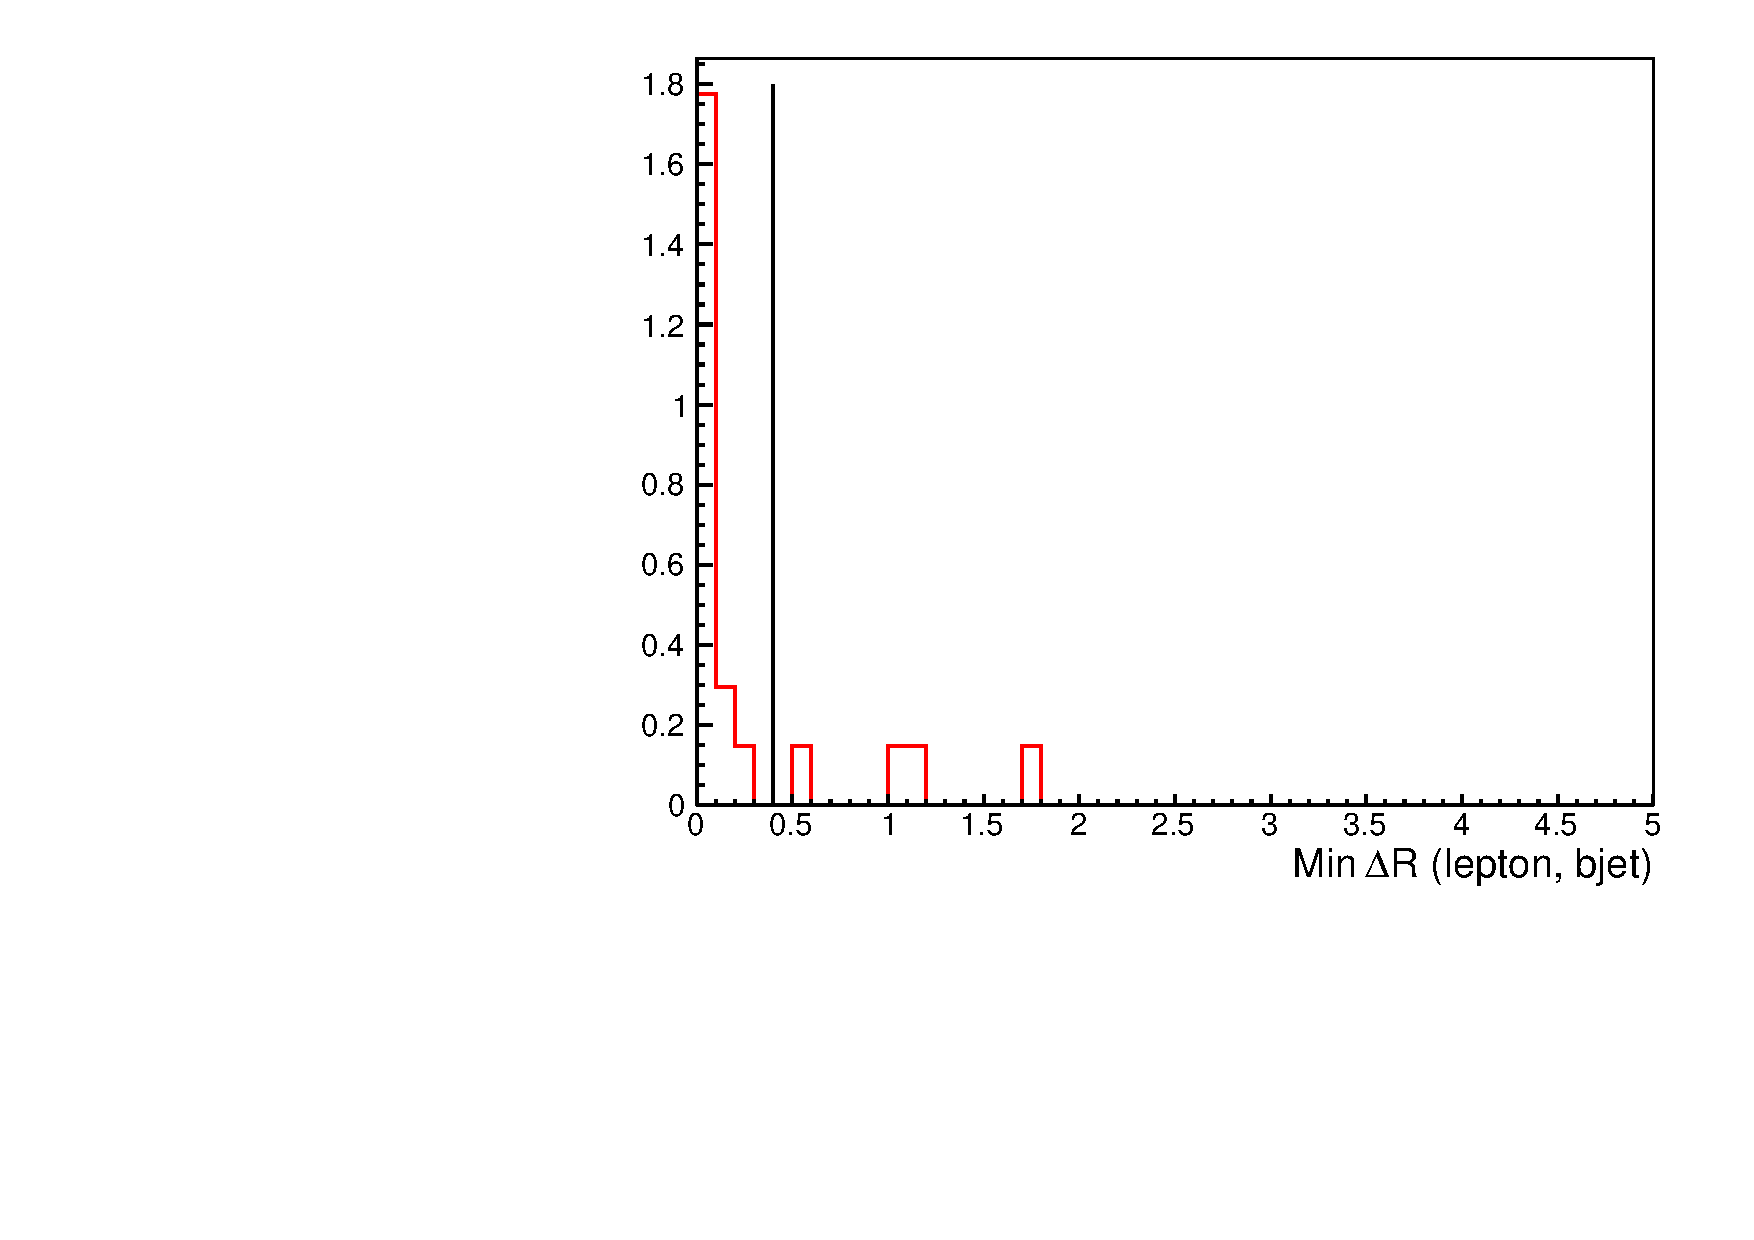
\includegraphics[width=0.6\linewidth, height=0.4\linewidth]{figs/bjetlepton.pdf}
\caption{ Minimum $\Delta R$ between the lepton and the b-tag jet in \ttbar decays.\label{fig:ttbar_residual}}
\end{center}
\end{figure}




 





\section{Acceptance Systematics}
\label{sec:systematic}
Systematic uncertainties arise from uncertainties on event selections expected in simulation 
compared to the actual performance of  the detector. 
As this search is in many ways similar to the inclusive same-sign dilepton search~\cite{ssnote2011}, 
our treatment of efficiency systematics parallels the one in that analysis.
In this section, we briefly summarize those results, and
describe the uncertanities due to the b-tagging requirement.

The only new source of systematics in this analysis is from the uncertainty on the
b-jet tagging efficiency.
As already mentioned in Section~\ref{sec:bjetSF}, this uncertainty
is 4 (14)\% for jets with $\pt<240 (>240)~\GeV$.
As an illustration of the b-jet momentum distribution,
we compare them in Fig.~\ref{fig:lm9ttbar} for  \ttbar\ events (before the same-sign requirement)
and for the LM9 cMSSM SUSY benchmark point.\footnote{
The LM9 point is defined by the common scalar mass (m0) $ = 1.45$ TeV, 
the common gaugino mass (m1/2) = 175 GeV, the ratio of the Higgs expectation
values (tan$\beta)  = 10$, tri-linear coupling (A0) = 0 and the  sign of the Higgsino mass parameter ($\mu) > 0$. 
}
While most of the b-jets from \ttbar\ are below 240~\GeV, those from LM9
have a large contribution from higher momenta.
Our target searches include final states with two or more b-quark jets.
This means the efficiency to select two b-jets, as well as its uncertainty
varies among the signal final states considered
\begin{itemize}
\item same-sign top pair production, as from $Z^\prime$ exchange,
	is similar in topology to that of the opposite-sign \ttbar\ production
	and has only two b-jets in the final state with most of them with $\pt<240~\GeV$.
	The b-tagging efficiency is then approximately 10\%
	and the corresponding per-event scale factor is $0.922 \pm 0.092$.
\item direct sbottom pair production has two b-jets in the final state
	with a large fraction of b-jets with $\pt>240~\GeV$.
	The b-tagging efficiency scale factor is still 0.922, but its uncertainty
	varies among the signal model points from as low as 10\%
	to as high as 30\%.
	This uncertainty is evaluated event-by-event and then point-by-point in the limit setting procedure.
\item gluino pair production with stops in the final states considered
	here all have four b-jets in the final state.
	Now the efficiency scale factor changes as well
	depending on the number of b-jets in the acceptance.
	This is evaluated event-by-event and point-by point in the limit setting procedure.
\end{itemize}


\begin{figure}[htb]
\begin{center}
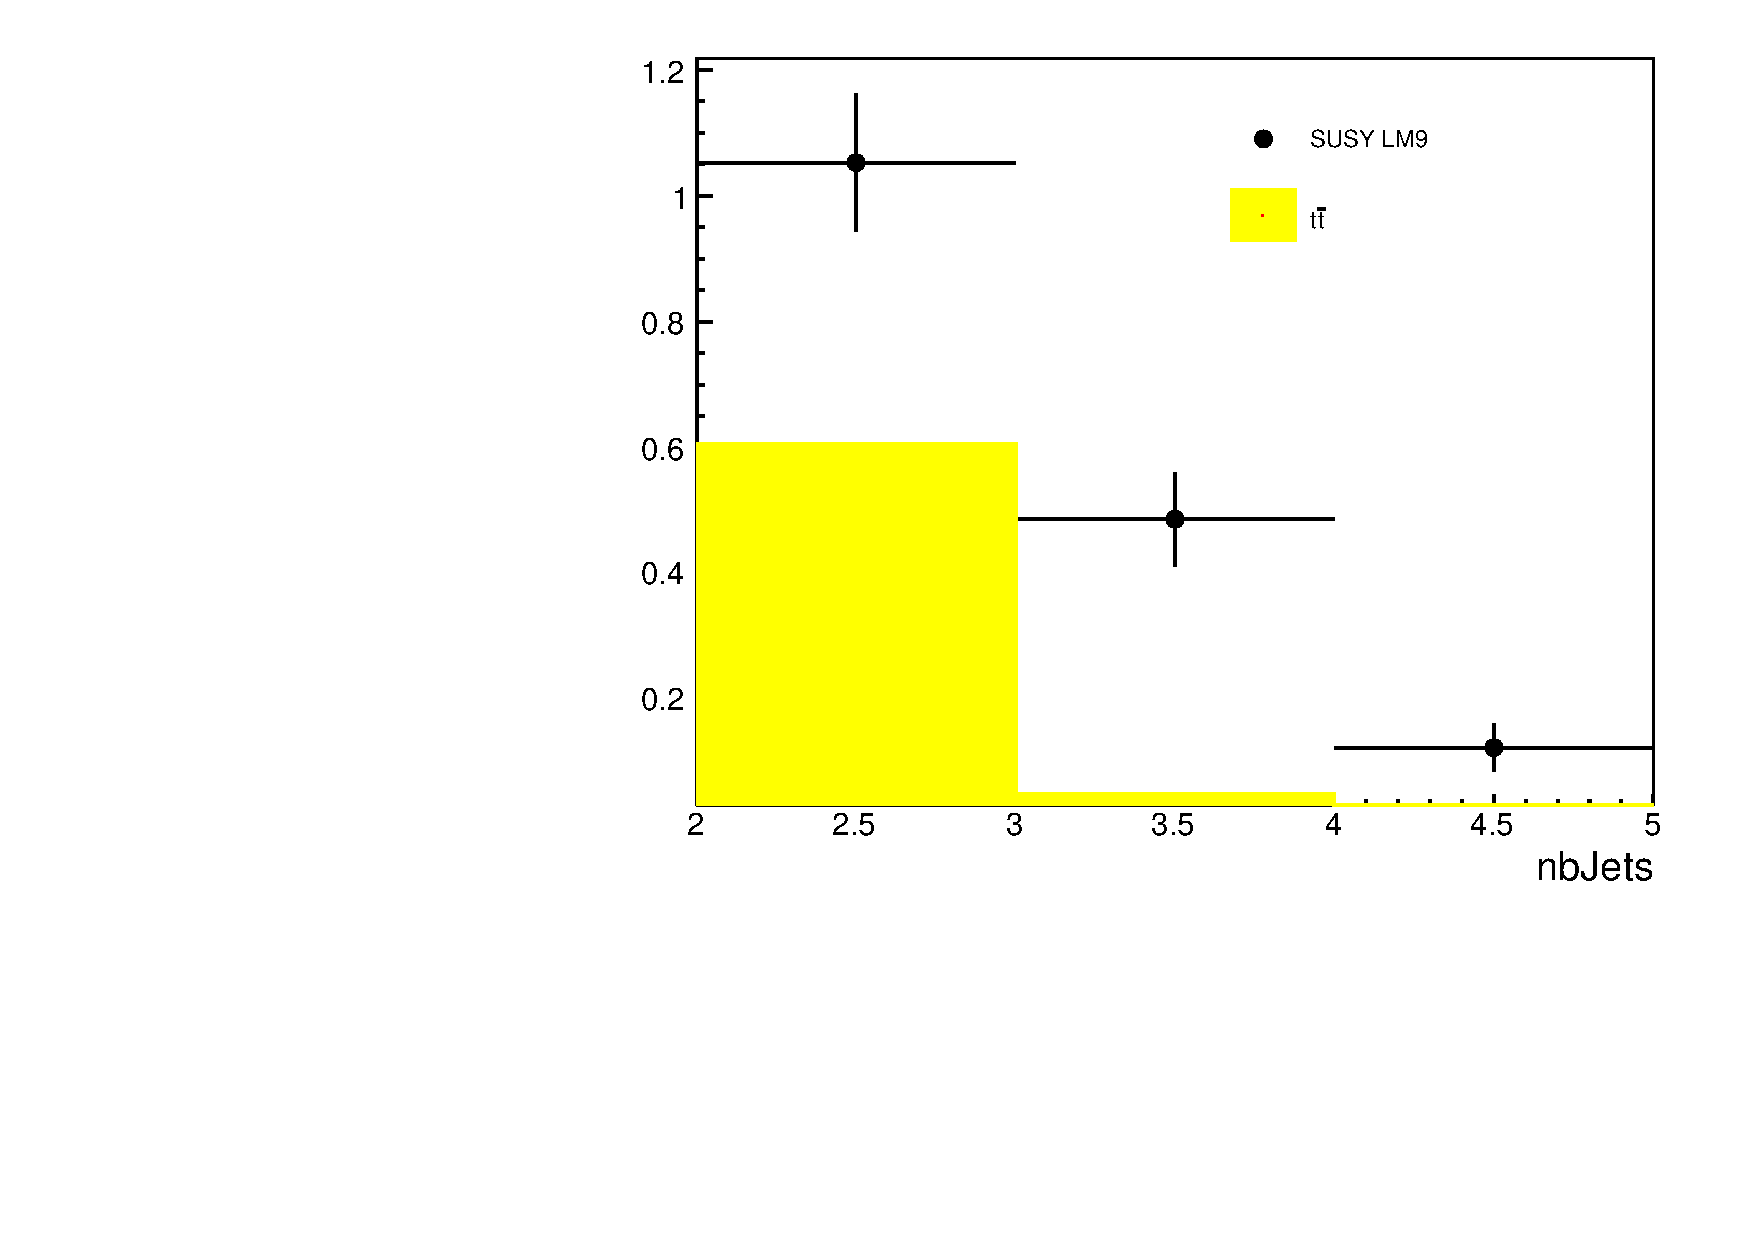
\includegraphics[width=0.48\textwidth]{figs/lm9.pdf}
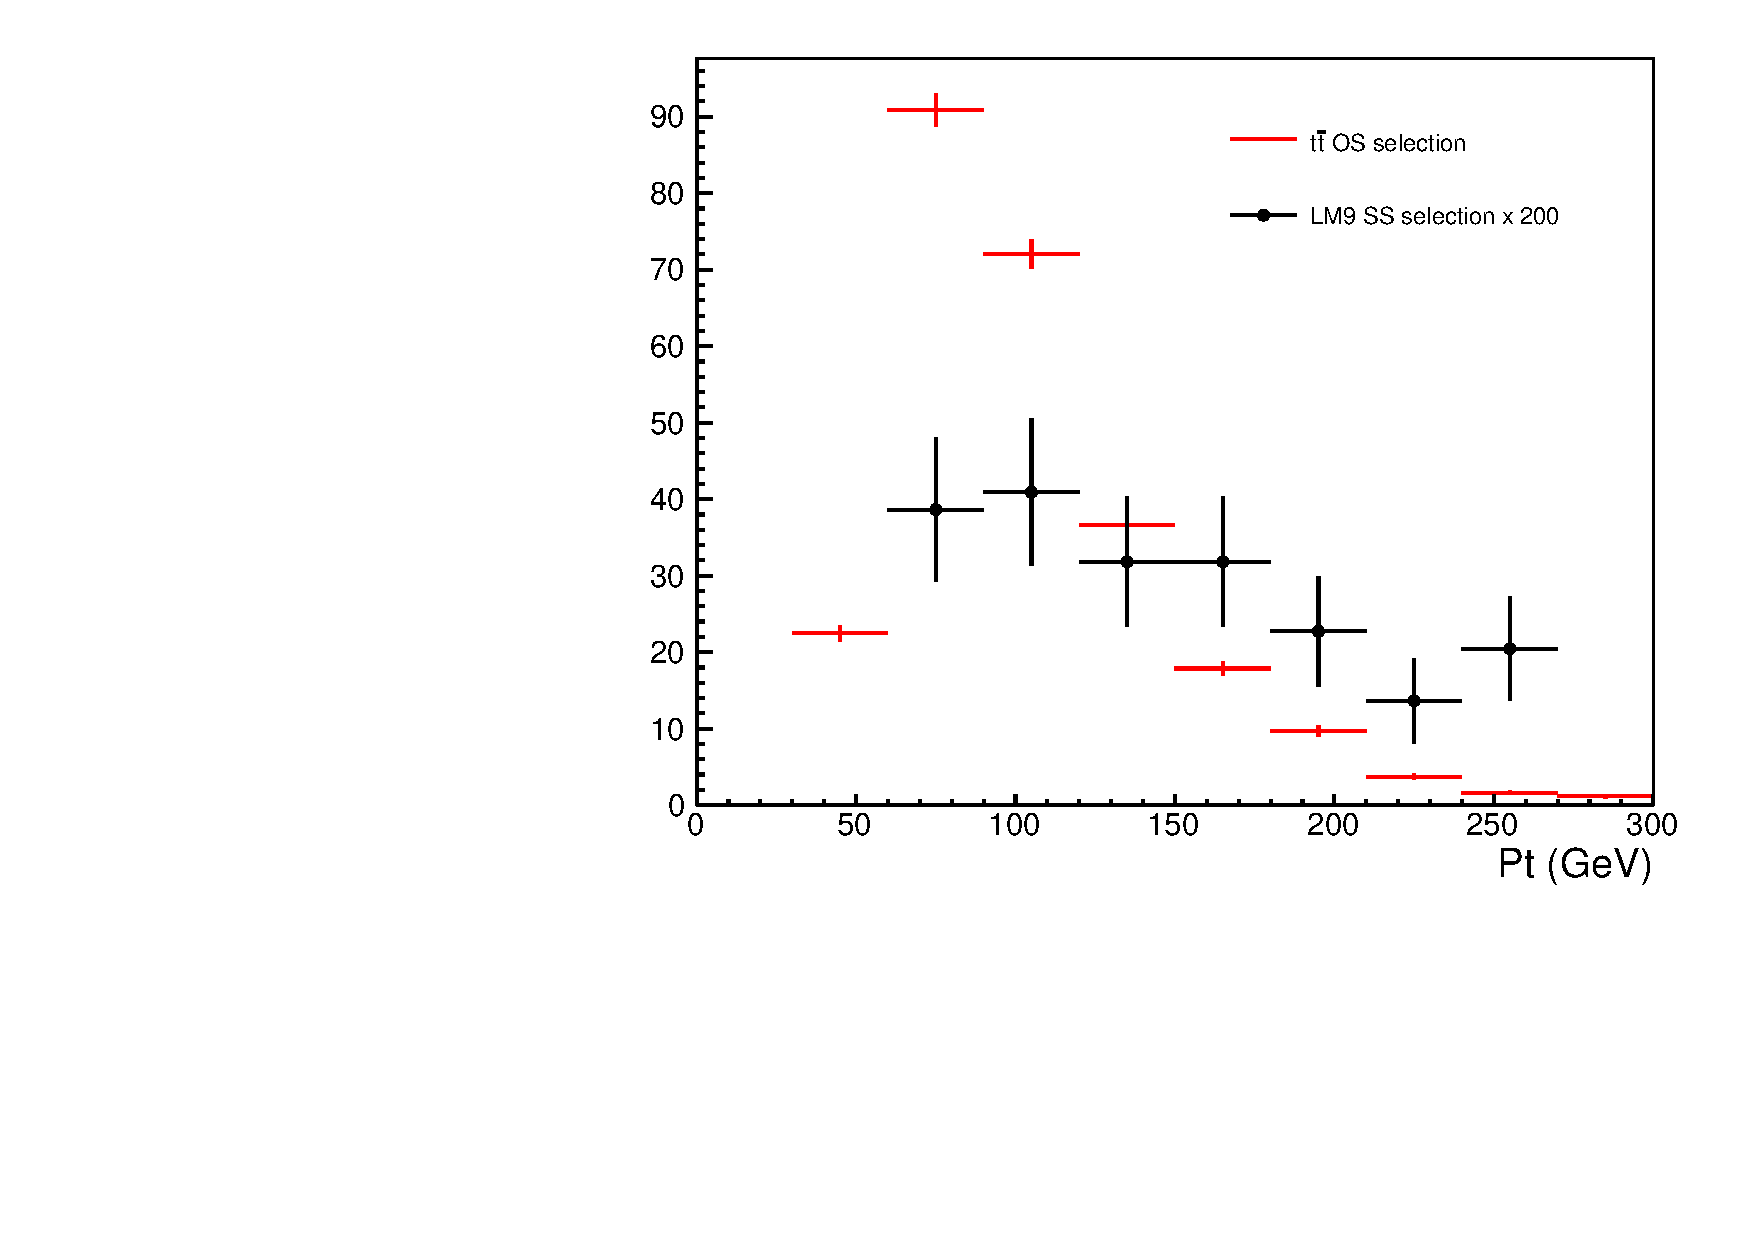
\includegraphics[width=0.48\textwidth]{figs/bjetleading.pdf}
\caption{ Differential distributions of leading b-tag jet $\pt$ for the 
LM9 benchmark point and \ttbar\ simulations.
The normalization is arbitraty.\label{fig:lm9ttbar}}
\end{center}
\end{figure}


A summary of systematic uncertainties is given in Table~\ref{tab:systSumm}.
Here the b-tagging systematics is applicable only to the same-sign top production signature.

\begin{table}[h]
\begin{center}
\caption{\small\label{tab:systSumm}Summary of systematic uncertainties on the signal selection and
expectation. 
Reported values are fractional, relative to the total cross section.
The energy scale, b-tagging, and PDF uncertainties are calculated separately in every model point.
These uncertainties quoted here are relevant to the $Z^\prime$ model.}
\begin{tabular}{lcccc}\hline
Source 					& $ee$		& $\mu\mu$		& $e\mu$	& all 	\\ \hline
Lepton selection			& 12\%		& 12\%			& 11\%		& 11\% 	\\
Energy scale				& 8\%		& 8\%			& 8\%		& 8\% 	\\
ISR/FSR and PDF				& 2\%		& 2\%			& 2\%		& 2\% 	\\
b-tag selection                         & 8\%          	& 8\%                   & 8\%           & 8\% 	\\
Total without luminosity		& 17\%		& 17\%			& 17\%		& 17\%	\\ \hline
Integrated luminosity			& 4.5\%		& 4.5\%			& 4.5\%		& 4.5\%	\\ \hline
Total 					& 17\%	 	& 17\%	 		& 17\% 		& 17\% 	\\
\hline
\end{tabular}
\end{center}
\end{table}

\subsection{Event-by-Event B-tagging scale factor and associated systematic uncertainty}
We evaluate an event-by-event btagging scale factor ($SF_{\rm event}$) as follows:

\begin{itemize}
\item for each MC event passing the event selection we start
from the scale factors $SF_i$ associated with the two or more
tagged jets.  Note that $SF_i$ can in principle be a function 
of jet $\eta$, $\pt$, etc.  Following the btag group recommendations,
for now it is taken as a constant: $SF=0.96$.

\item For events with two btagged jets: $SF_{\rm event}=SF^2$.

\item For events with three btagged jets: $SF_{\rm event}=SF^3 + 3SF^2(1-SF)$.

\item For events with four btagged jets: $SF_{\rm event}=SF^4 + 4SF^3(1-SF) + 6SF^2(1-SF)^2$.
\end{itemize}

Note that the procedure above would not work if $SF>1$, but this is not an issue
since $SF=0.96$.
It also implicitely assumes that all btags are from b-quarks.  For the models under 
consideration, we have verified that the MC contribution to the acceptance from 
events that need at least one tag from $udsgc$ in order to pass the $\ge$ 2 tags 
requirements is small.  For example, in the $Z'$ model, this contribution is
only $\approx$ 4\%.  Note that the bias in $SF_{\rm event}$ due to the improper traeatment
these events is 4\% times some quantity proportional to the difference in scale 
factors between $b$-jets and $usdgc$ jets.  Therefore, it is $<<$ 4\% and we think
can be ignored.  

In order to calculate the uncertainty ($\delta SF$) on the event-by-event $SF_{\rm total}$,
we also need the single jet btagging efficiency ($\epsilon$).  
We do not need a very precise value for $\epsilon$, since the uncertainty $\delta SF$ is 
only weakly dependent on it.  We take $\epsilon = 0.643$, independent of $\pt$
and $\eta$ for jets of $|\eta| < 2.5$.  The uncertainty on $\epsilon$ is 
the same as that on the scale factors, $\delta \epsilon = 4\% (14\%)$ (relative)
for $\pt < 240$ GeV ($> 240$ GeV).
The procedure is the following:
\begin{itemize}

\item For each event passing the requirements at RECO level, we look at the status=3 information
and we calculate the total probability ($p$) of tagging two or more jets, and 
its uncertainty ($\delta p$).

\item The calculation of $p$ and $\delta p$ is based on the number of status=3 b-quarks
of $\pt > 40$ GeV and $|\eta| < 2.5$.  

\item An event with two reconstructed btags can have $<$ 2 such status=3 b-quarks.  This 
is rare and happens for example when a 39 GeV b-quark is reconstructed as a 41 GeV
b-jet.  In these cases we calculate $p$ and $\delta p$ assuming that there are 
two 40 GeV b-quarks at status=3.

\item The uncertainty associated with the event is then $(\frac{|\delta p|}{p}) SF_{\rm event}$.

\end{itemize}

The probabilities $p$ are calculated as follows ($N$ here is the number of status=3 b-quarks
and we write the equations without the assumtion that $\epsilon$ is constant):

\begin{itemize}

\item $N=2$:~~~~$p = \epsilon_1 \epsilon_2$.

\item $N=3$:~~~~$p = \epsilon_1 \epsilon_2 + \epsilon_1 \epsilon_3 + \epsilon_2 \epsilon_3 -
2\epsilon_1 \epsilon_2 \epsilon_3$.

\item $N=4$:~~~~$$p = \prod{\epsilon_i}~~~+~~~\sum_j{(1-\epsilon_j)\prod_{i \ne j}{\epsilon_i}}
~~~+~~~\sum_{j<k}{(1-\epsilon_j)(1-\epsilon_k)\prod_{i \ne j,k}{\epsilon_i}}$$



\end{itemize}

The uncertainties $\delta p$ are calculated from the equations above assuming full 
correlation between jets, {\em e.g.}, for $N=2$ we have 
$\delta p$ = $\delta \epsilon_1 \cdot \epsilon_2 + \delta \epsilon_2 \cdot \epsilon_1$, etc.


\section{Results on Inlcusive Signature Search}
\label{sec:inclresults}

{\bf This section is missing two things. First, we will add a \met\ vs $H_T$ plot that shows the data and
one of the models overlayed. Second, we will add a summary of the events we see. 
}

We see 2 (1) events in the high-$p_T$ (low-$p_T$) analysis with a predicted background of
1.0$\pm$ 0.8 (0.5$\pm$ 0.7).
In absence of any significant deviation from the predicted background, we set 95\% CL. on the number of observed events. 
Two statistical methods have been used for the upper limit. 
Both methods assume the uncertainties on signal and background are un-correlated and use a log-normal distribution for error pdfs. 

The first method used to compute the upper limit is based on the Bayesian method~\cite{bayesian}.
A posterior probability $p(r)$ is used as a function of the signal strength $r = \sigma/\sigma_{SM}$ 
assuming a uniform prior for the signal strength $r$ integrating the nuisance parameters associated with the uncertainties.
The upper limit at 95\% confidence level is then determined by integrating $p(r)$ to determine $r'$, 
which satisfies $\int_{r'}^{\inf} p(r) dr = 0.05$.

We use the hybrid frequentist-bayesian $CLs$ approach~\cite{CLSxx} as the second method. 
Although the two statistical approaches are not equivalent, in this case we get similar results. 

\begin{itemize}
\item Upper limit using high-$p_T$ analysis at 95\% CL. with 24\% signal systematic error using Bayesian approach = 6.1  
\item Upper limit using high-$p_T$ analysis at 95\% CL. with 24\% signal systematic error using $CLs$ = 5.8  
\item Upper limit using low-$p_T$ analysis at 95\% CL. with 24\% signal systematic error using Bayesian approach = 4.8  
\item Upper limit using low-$p_T$ analysis at 95\% CL. with 24\% signal systematic error using $CLs$ = 4.6  
\end{itemize}

We use 6.1 and 4.8 events as the upper limit for the rest of this document for high- and low-$p_T$ analyses.

\section{Searches for Specific Models}
\label{sec:stampCollecting}

Our signature, two isolated same-sign leptons plus, at least two b-tagged jets, and \met, 
is common to many different new physics scenarios.
Here we refine our analysis to define dedicated signal regions for a few of these scenarios,
and provide 95\% C.L. upper limits on their respective model parameter space.


\subsection{Same sign top production due to a $Z'$}
\label{sec:sstops}

This is an extension of the 2010 CMS published CMS analysis\cite{sstop}.
The main difference is that here in order to improve the signal-to-noise
we require two b-tagged jets.  This would not have made sense in 2010, since 
at the time the integrated luminosity was low enough that the analysis was almost
background free without requiring b-tags.

\subsubsection{Theoretical Discussion, $Z'$ model}

Recent measurements of the inclusive forward-backward $t\bar{t}$ production 
asymmetry ($A_{FB}$) from the 
Tevatron experiments show deviations from the standard model 
(SM) expectations~\cite{d0:fwtop, cdf:fwtop1, cdf:fwtop2}.
% The largest (3$\sigma$) deviation~\cite{cdf:fwtop2} is found 
% to be in the region of high invariant mass with $M_{t\bar{t}} >  450$ GeV. 
Several attempts have been made to explain this asymmetry~\cite{fcnczprime, Buckley, Gresham, zoltan}. 
One of the most natural ways to induce such an asymmetry would be through
Flavor Changing Neutral Currents (FCNC) in the top quark sector. 
The forward-backward asymmetry in $u\bar{u} \to t\bar{t}$ would then be generated
by t-channel exchange of a new massive $Z'$ boson that couples chirally to
$u$ and $t$ at the same vertex, as shown in Fig.~\ref{fig:ttbaras}~\cite{fcnczprime}.
The same type of interaction would also give rise to same-sign top pair production, 
as illustrated in Fig.~\ref{fig:tchannel} and Fig.~\ref{fig:schannel}. 
In this case, the initial state involves two $u-$quarks and 
thus the cross section at the LHC is enhanced due 
to the large valence quark parton density of the proton. 

\begin{figure}[htb]
\begin{center}
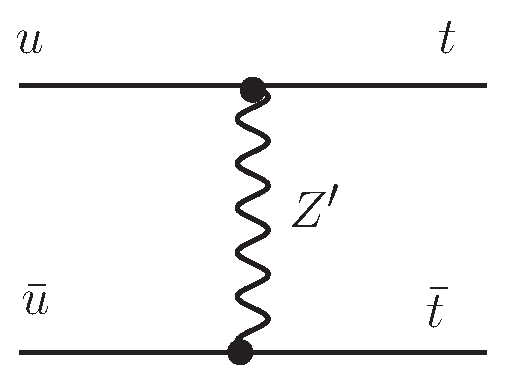
\includegraphics[width=0.35\linewidth, height=0.25\linewidth]{figs/ttbar_Z.pdf}
\caption{ Diagram for $t\bar{t}$ production induced by $Z'$ exchange which
can generate a forward-backward asymmetry. \label{fig:ttbaras}}
\end{center}
\end{figure}

\begin{figure}[htb]
\begin{center}
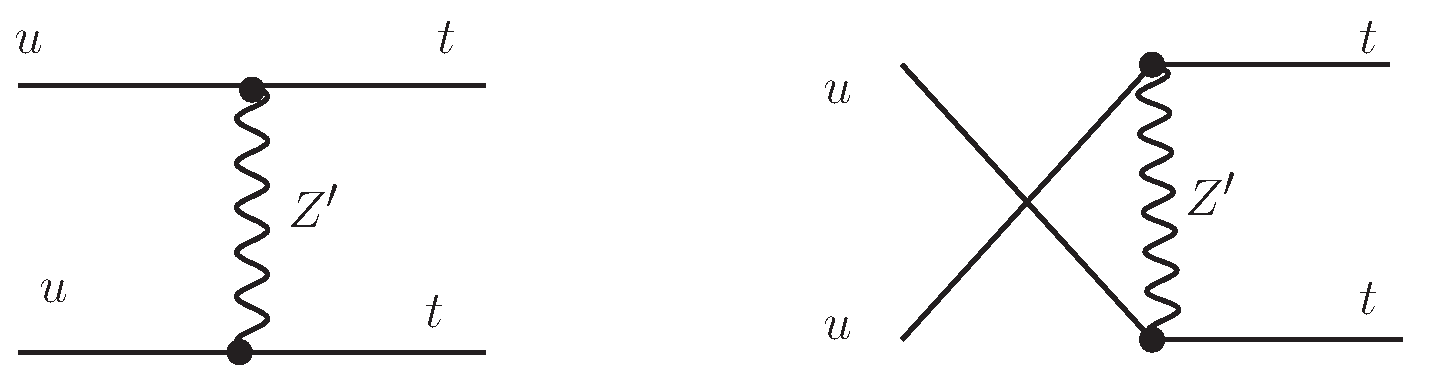
\includegraphics[width=0.7\linewidth, height=0.2\linewidth]{figs/sstop1.pdf}
\caption{ Diagrams for $tt$ pair production induced by $Z'$ exchange in the t-channel. 
\label{fig:tchannel}}
\end{center}
\end{figure}

\begin{figure}[htb]
\begin{center}
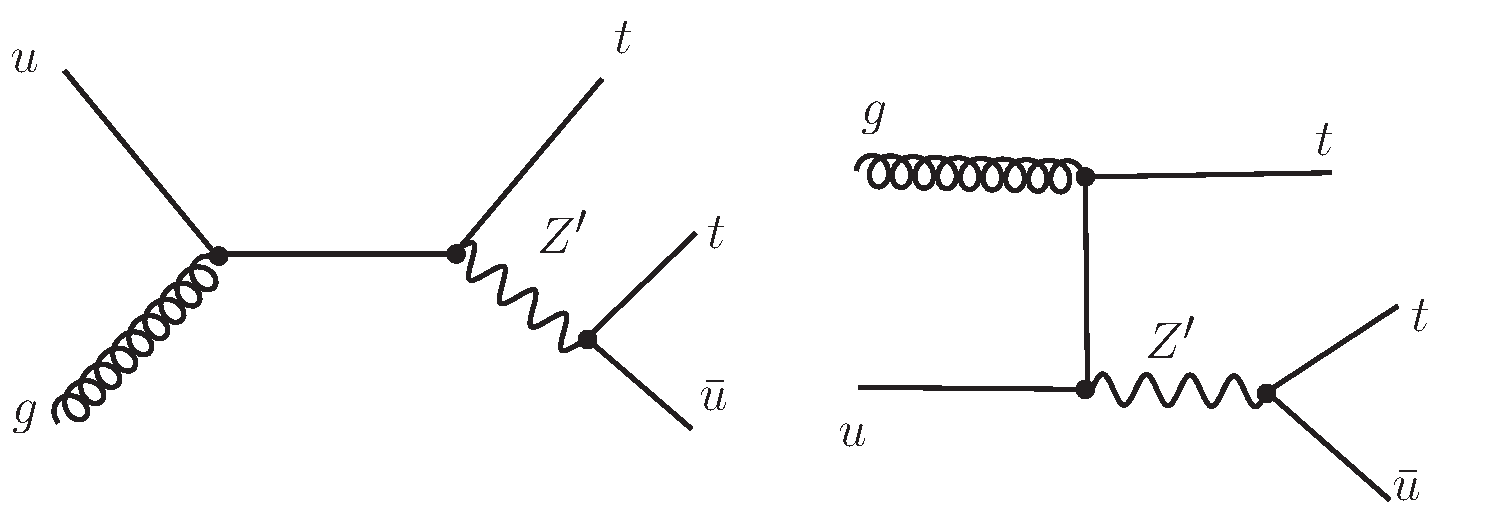
\includegraphics[width=0.7\linewidth, height=0.25\linewidth]{figs/sstop2.pdf}
\caption{ Diagrams for $tt\bar{u}$ production induced by $Z'$ exchange in the s-channel 
\label{fig:schannel}}
\end{center}
\end{figure}


We consider the model of Reference~\cite{fcnczprime}.  
The relevant $u-t-Z'$ interaction term in the Lagrangian is:

\begin{equation}
\label{eqn:L_berger}
  \mathcal{L} = g_W \bar{u} \gamma^\mu (f_L P_L + f_R P_R)tZ'_\mu + h.c
\end{equation}

where $g_W$ is the weak coupling strength. The left-handed coupling is set to $f_L = 0$, due 
to the $B_d-\bar{B_d}$ mixing constraint~\cite{Cao}. 
The right-handed coupling $f_R$ and the $Z'$ mass are free parameters in the model.
Within this model there is a narrow range of parameter space
consistent with the TeVatron measurements of $\sigma(p\bar{p} \to t\bar{t})$ 
and $A_{FB}$, which is not excluded by direct searches for same sign tops.
This region is illustrated in Fig.~\ref{fig:berger_limit}.

% Fig.~\ref{fig:tchannel} shows the t-channel exchange diagrams that can lead to the same-sign $tt$ final state. 
% As expected the coupling appears twice in the Feynman diagrams, thus the predicated rate is proportional to $f_R^4$. 

\begin{figure}[htb]
\begin{center}
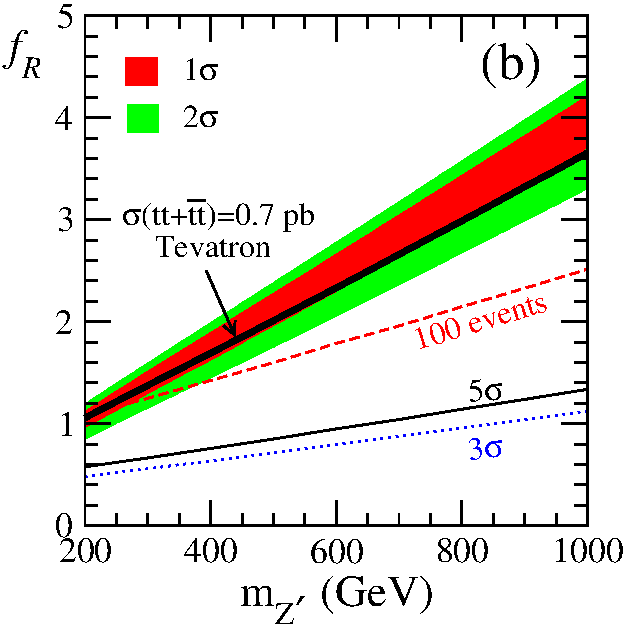
\includegraphics[width=0.4\linewidth]{figs/berger_limit.pdf}
\caption{\protect From Reference~\cite{fcnczprime}; the shaded area covers the parameter
space consistent with the $A_{FB}$ and $\sigma(t\bar{t})$ from the Tevatron;
The line indicated by the arrow shows the Tevatron limit inferred by the authors
from same sign top searches at the Tevatron; the remaining lines represent the
expectations of Reference~\cite{fcnczprime}.
for LHC searches in 1 fb$^{-1}$. \label{fig:berger_limit}}
\end{center}
\end{figure}

Monte Carlo events for this model were generated using Madgraph in the same way as 
for the 2010 analysis (see Reference~\cite{ttAN}).



\subsubsection{Signal region definition for same sign top from $Z'$}
\label{sec:sstopsigdefinition}
In this study we search for same-sign dileptons originating from $tt$ 
or $ttj$ pair production as described above.  At the LHC $uu \to tt$ 
dominates over $\bar{u}\bar{u} \to \bar{t}\bar{t}$, thus we concentrate
on same-sign positive leptons.  The \met~~and $H_T$ cuts are typical 
of a dilepton top analysis: two or more jets of $P_T>40$ GeV, 
$\met > 30$ GeV and $H_T > 80$ GeV.  This corresponds to Table~\ref{tab:yieldBase_pp}:
5 events observed and 4.42 $\pm$ 0.80 $\pm$ 1.39 expected from background.

\subsubsection{Limits on the $Z'$ model}
\label{sec:sstopslimits}
Using the results from Section~\ref{sec:sstopsigdefinition}, we set 
a limit at 95\% CL of 7.2 events using the CL$_{\rm S}$ method.
The expected limit is 6.4 events.
% $7.8^{+3.6}_{-3.1}$ events.
In the MC we find $Acc \times Eff \times BR = 0.00233$, independent of $Z'$ mass. 
This results in an upper limit on the cross-section of 0.67 pb.
The limit includes uncertainty
on JES (12\%), btagging (10\%), lepton efficiencies (11\%), luminosity (4.5\%),
and PDF (3\%).

The cross-section limit is turned into an exclusion limit in the $m(Z')$ vs $f_R$
plane using the LO calculation of the $pp \to tt$ cross-section in this model.
This is shown in Figure~\ref{fig:sstopexclusion}, together with the corresponding
plot from the 2010 analysis.  The region of parameter space favored consistent 
with the Tevatron measurements of $A_{FB}$ is excluded.


For $M_{Z'} >> M_{\rm top}$ the Lagrangian of equation 1 is 
equivalent to 
$\mathcal{L} = -\frac{1}{2}\frac{C_{RR}}{\Lambda^2}
 [\bar{u} \gamma^\mu t][\bar{u} \gamma_{\mu} t] + h.c.$~\cite{cdfth2},
with $\frac{C_{RR}}{\Lambda^2} = \frac{2 g_W^2 f_R^2}{M_{Z'}^2}$.
 Our limit on $f_R$, calculated for $M_{Z'}=2$ TeV, 
would then correspond to $\frac{C_{RR}}{\Lambda^2} < 0.6$ TeV$^{-2}$ at 
95\% confidence.  This is more stringent than the limit recently reported
by CDF: $\frac{C_{RR}}{\Lambda^2} < 3.7$ TeV$^{-2}$~\cite{cdflimit}.


\begin{figure}[htb]
\begin{center}
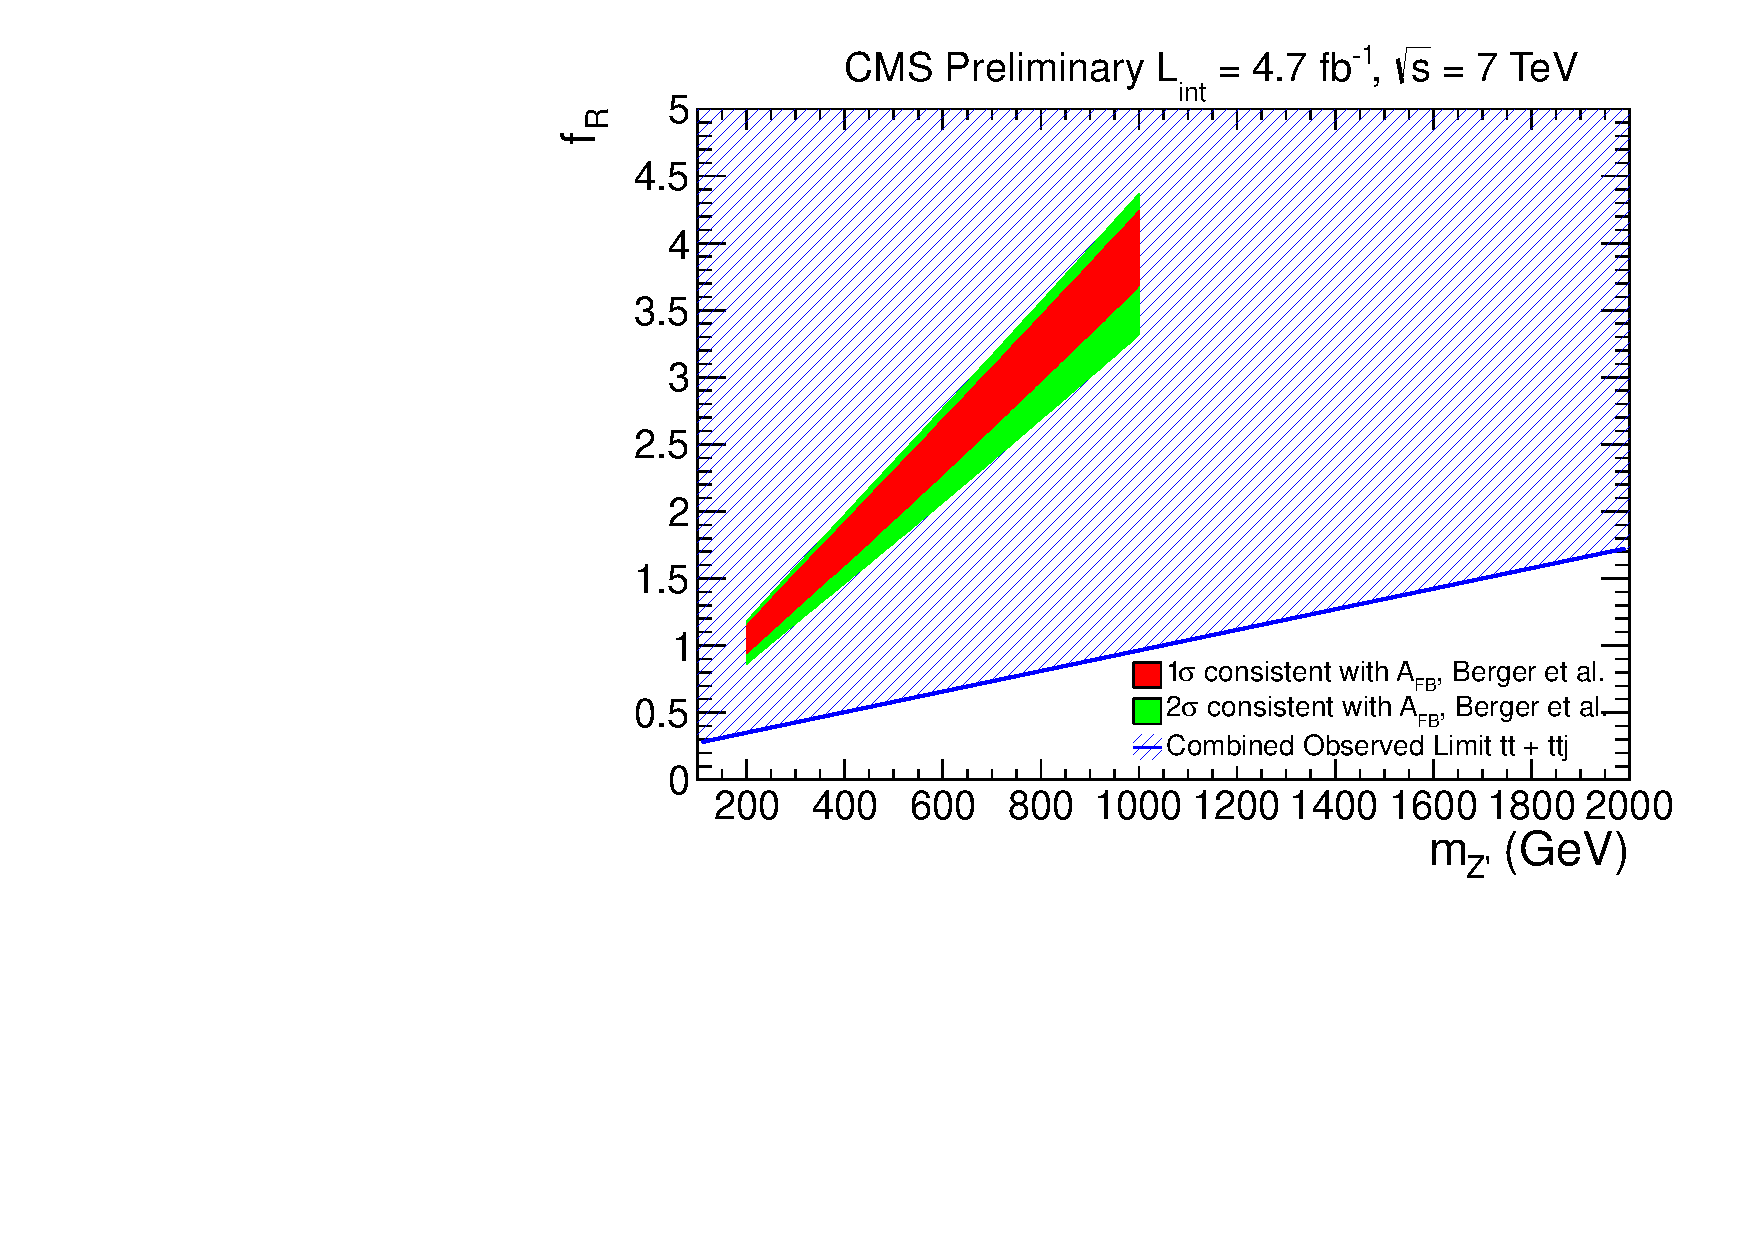
\includegraphics[width=0.45\linewidth]{figs/zprimecombined.pdf}
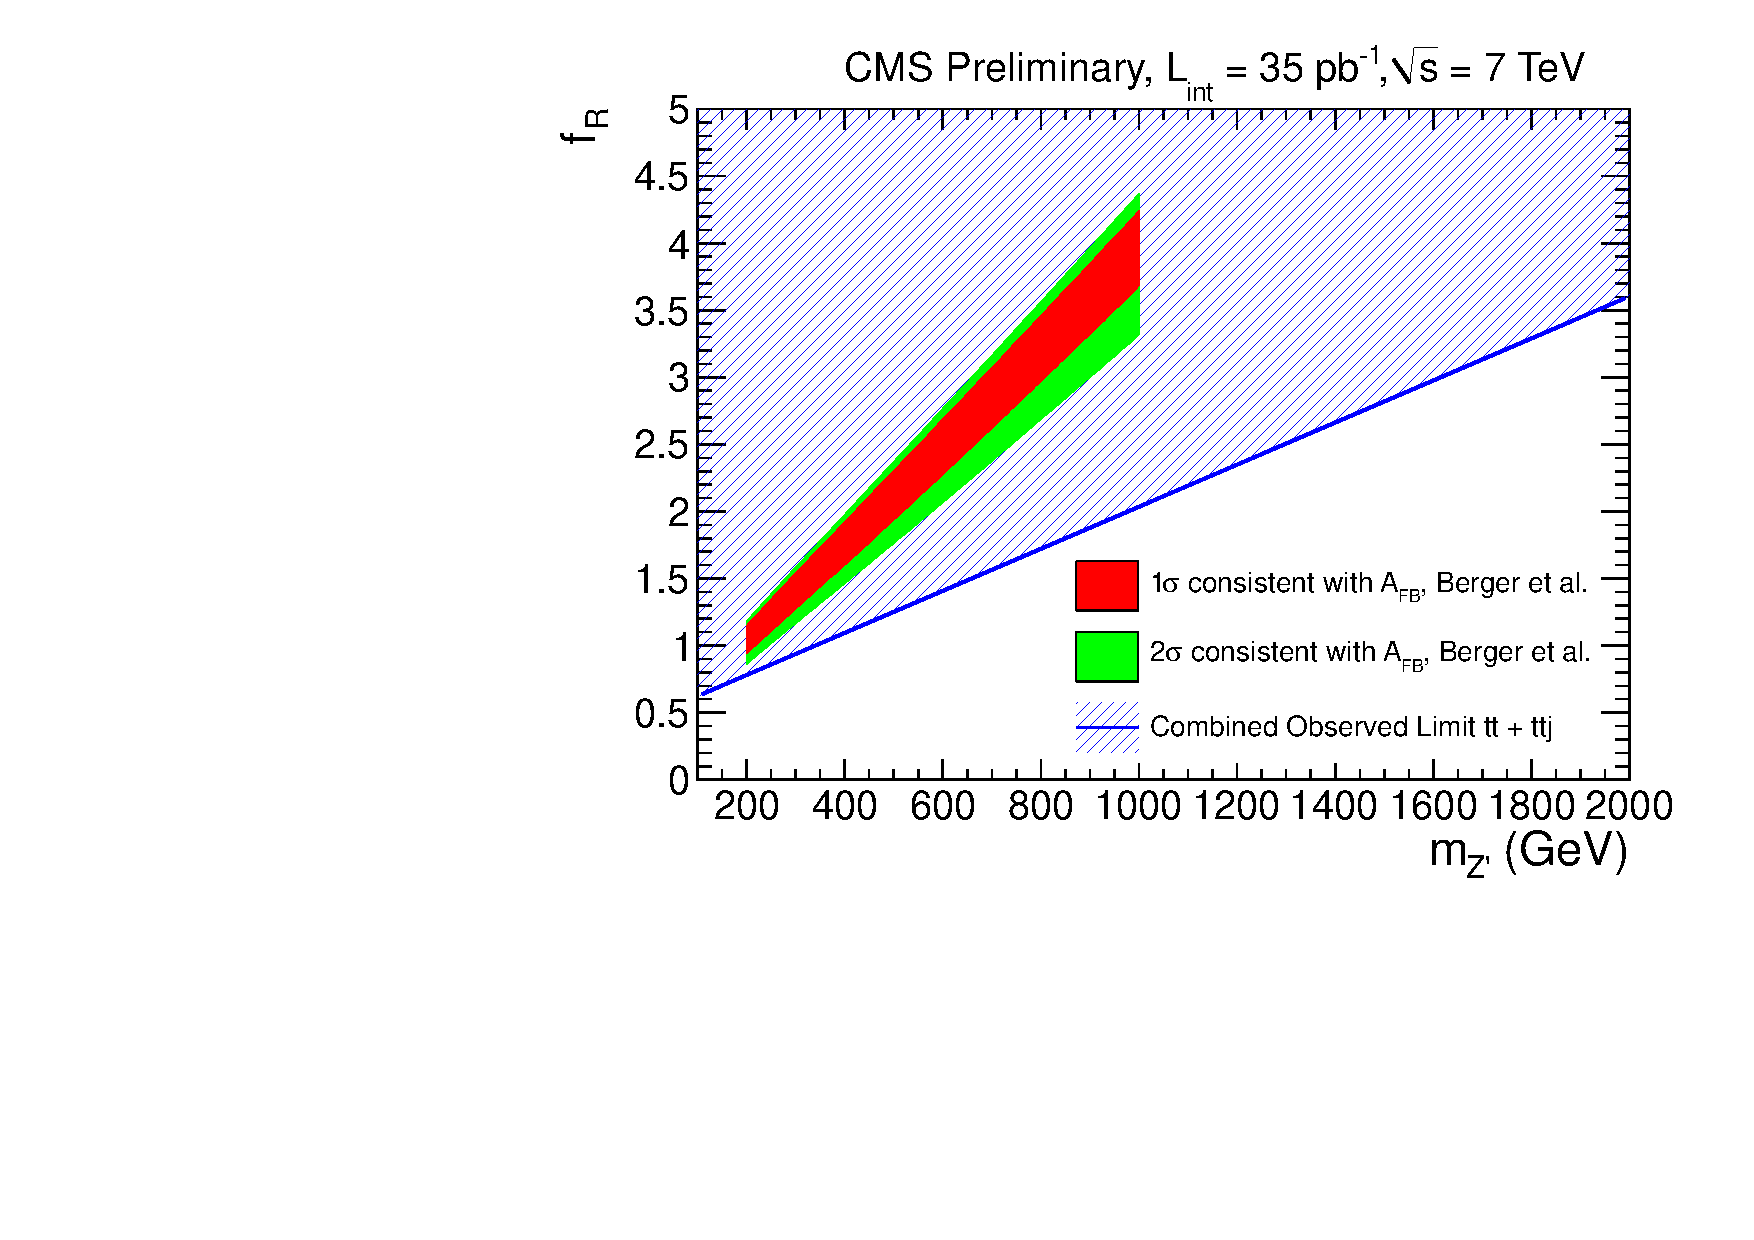
\includegraphics[width=0.45\linewidth]{figs/sscomb.pdf}
\caption{Exclusion regions from the 2011 analysis (left) and the 2010 analysis (right).
The exclusions are obtained using the LO cross-section for $tt$ production.  
Note that the cross-section is proportional to $f_R^4$.
\label{fig:sstopexclusion}}
\end{center}
\end{figure}

%\subsubsection{What is still missing for the $Z'$ model}
%\begin{itemize}
%\item Double check calculation of $\frac{C_{RR}}{\Lambda^2}$
%\item Double check acceptance numbers
%\end{itemize}


%\clearpage


\subsection{Maximally Flavor Violation Model (MXFV)}
\label{sec:mxfv}

\subsubsection{Theoretical discussion of MXFV}
\label{sec:mxfvtheory}

This is a model~\cite{mxflv1,mxflv2,mxflv3} with a new scalar 
SU(2) doublet field $\Phi_{FV} = (\eta^0,\eta^+)$ that couples the first and third 
generation quarks ($q_1,q_3$) via a Lagrangian term 
$\mathcal{L}_{FV} = \xi_{13} \Phi_{FV} q_1 q_3$.  Remarkably, it appears that this
model is largely consistent with constraints from flavor physics.

The model results in same sign top pairs in the final state as foolows
\begin{itemize}

\item Single $\eta^0$ production: $ug \to t\eta^0 \to tt\bar{u}, t\bar{t}u$

\item $\eta^0$ pair production: $u \bar{u} \to \eta^0 \eta^0 \to tt\bar{u}\bar{u},
uu\bar{t}\bar{t}, t\bar{t}u\bar{u}$

\item $\eta^0$ $t$-channel exchange: $uu \to tt$, $\bar{u}\bar{u} \to \bar{t}\bar{t}$
\end{itemize}

Monte Carlo events were generated using LHE files\cite{simplifiedModel} interfaced 
with Madgraph.  Madgraph was used to decay the top quarks in order to preserve 
spin-correlations.  The cross-sections at LO for same sign $tt$ pairs for the three
processes in the MXFV model is shown in Figure~\ref{fig:mxvxsec}.  The $t$-channel
process is the dominant for $\xi = 1$.  At smaller values of $\xi$, 
$ug \to \eta^0 \to tt\bar{u}$ becomes more important, since its cross-section 
varies as $\xi^2$, while in the $t$-channel case it goes as $\xi^4$.

\begin{figure}[htb]
\begin{center}
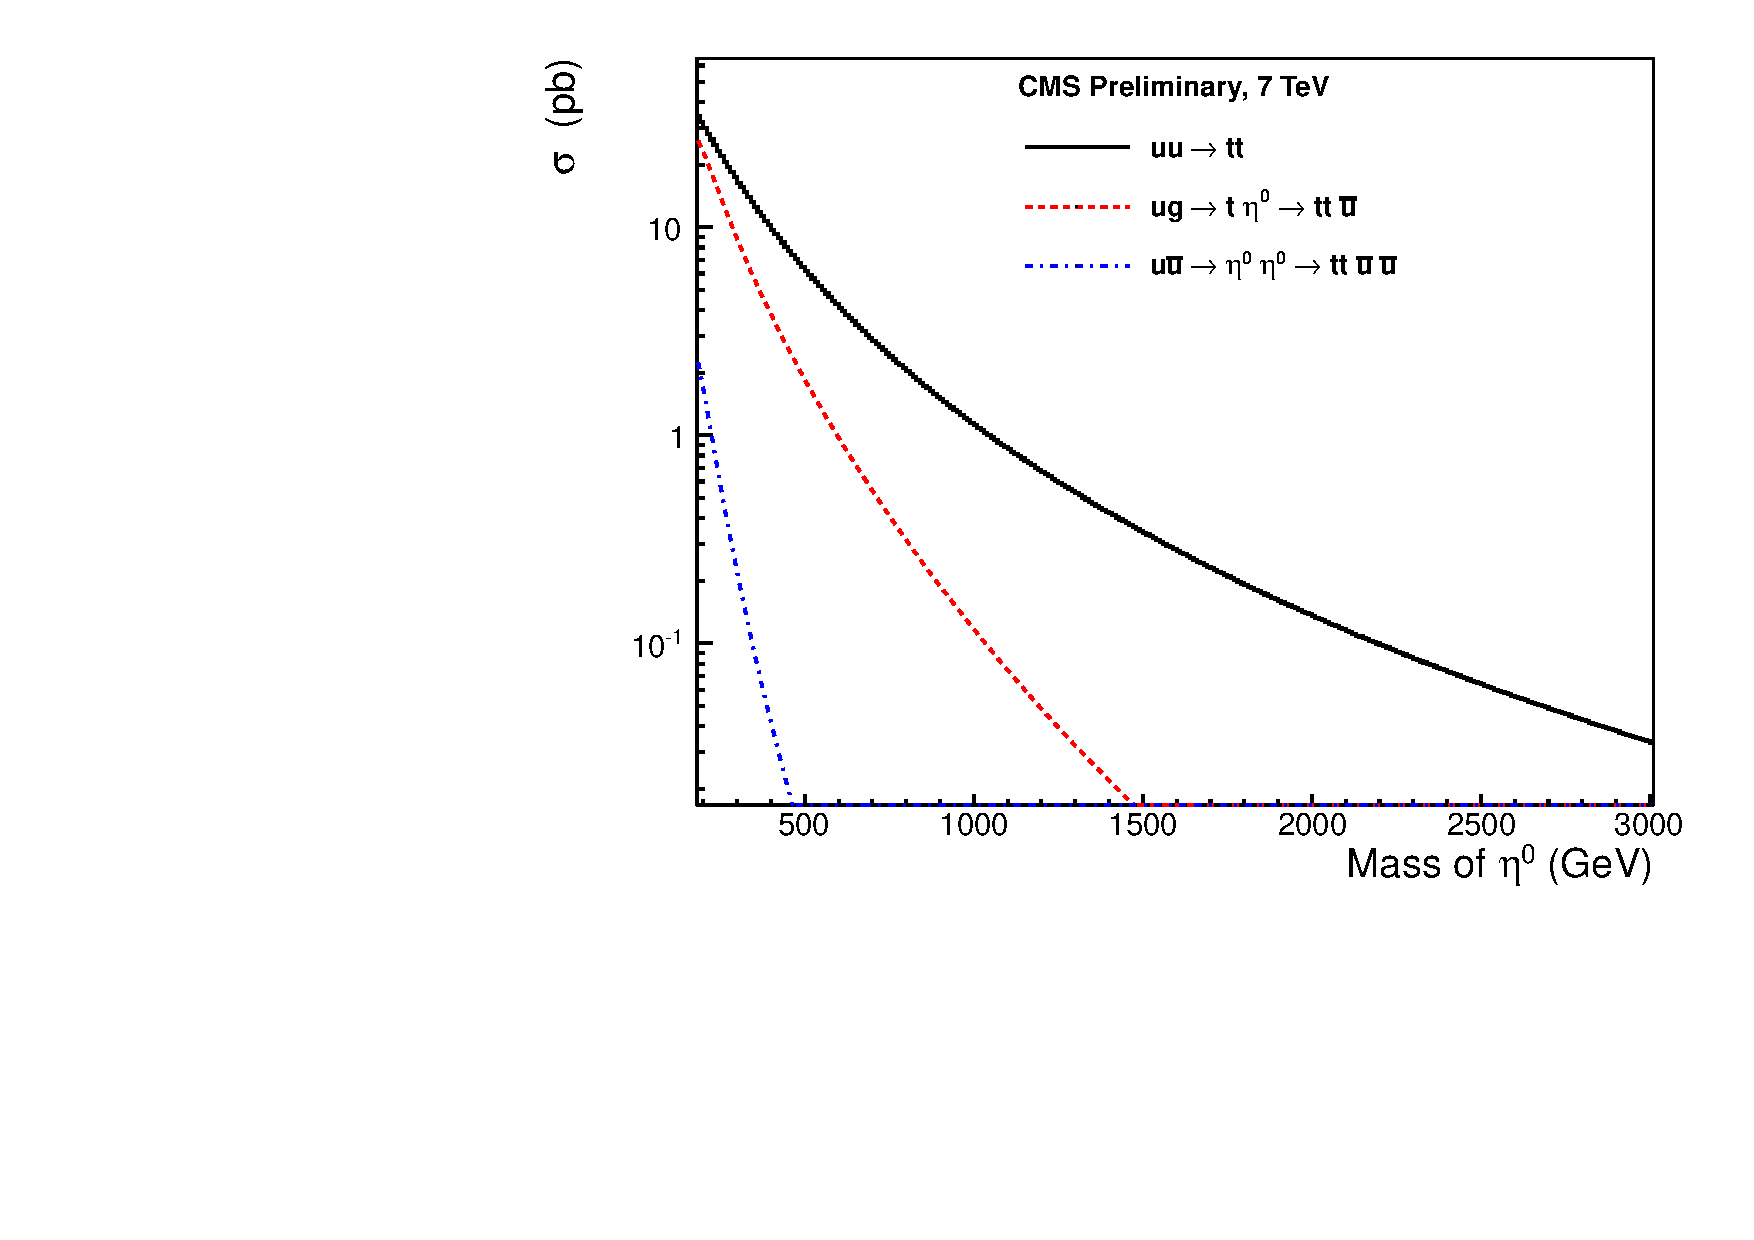
\includegraphics[width=0.55\linewidth]{figs/mxvxsec.pdf}
\caption{Cross section at LO for the $tt$ final state in the three MXFV modes
as a function of $\eta^0$ mass for $\xi = 1$.
\label{fig:mxvxsec}}
\end{center}
\end{figure}

\subsubsection{Signal region definition for the MXFV model}
\label{sec:mxfvdefinition}
The properties of the final state in this model are basically the same as in the $Z'$ model.
Thus, we use the same signal region definition (see Section \ref{sec:sstopsigdefinition}).


\subsubsection{Limits for the MXFV model}
\label{sec:mxfvlimits}
Our limits in the $\xi$-M($\eta^0$) plane are shown in 
Figure~\ref{fig:MxVExcl}.
They are calculated using the LO cross-section for this model.

\begin{figure}[htb]
\begin{center}
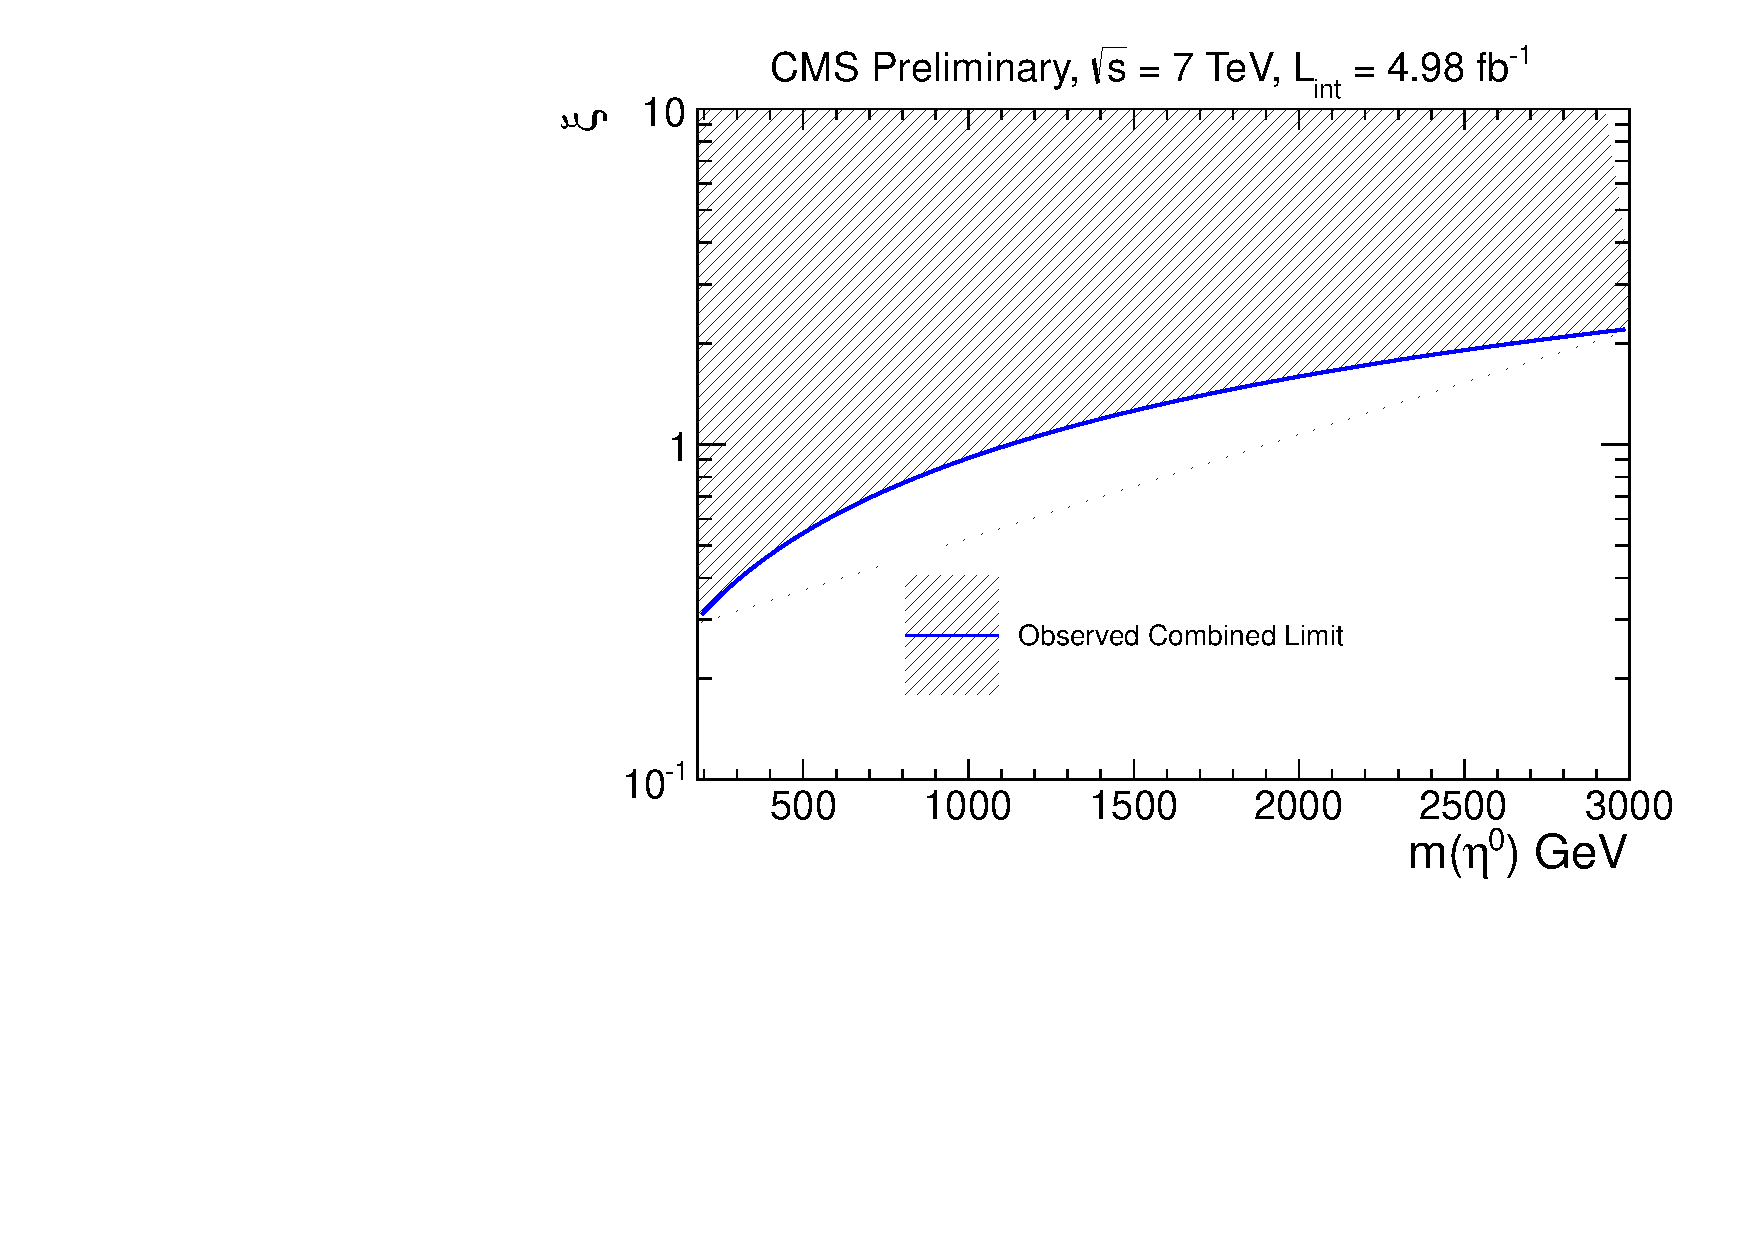
\includegraphics[width=0.45\linewidth]{figs/MxVExclCombined.pdf}
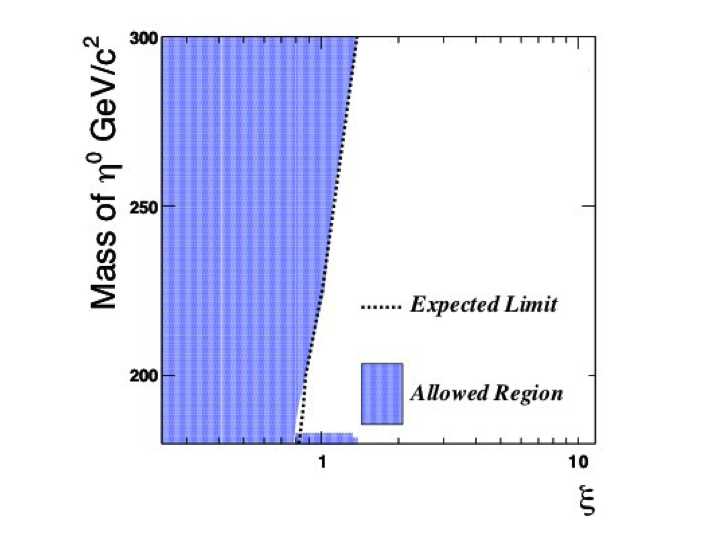
\includegraphics[width=0.45\linewidth]{figs/CDFlimit.png}
\caption{Limits in the $\xi$-Mass($\chi^0$) plane.  Left: CMS.  Right: CDF
\label{fig:MxVExcl}}
\end{center}
\end{figure}

%\subsubsection{What is still missing for the MXFV model}
%\begin{itemize}
%\item Need to include the $tt\bar{u}$ final state
%\item Rescale everything to take into account that the leptonic BR in MG is not quite right
%\item Signal Contamination effects (should be tiny)
%\item Prettify the exclusion plot, put CDF on same plot perhaps
%\end{itemize}



\subsection{$\widetilde{g} \to t\widetilde{t}$ Model}
\label{sec:firststopmodel}

\subsubsection{Theoretical discussion of the $\widetilde{g} \to t\widetilde{t}$ Model}
\label{sec:firststopmodeltheory}

This is an interesting model for stop pair production through gluino 
decays\cite{susyssbtags}\cite{susyssbtags2}\cite{wacker}\cite{naturalness4}.
It is a ``realistic'' and well-motivated 
model in the sense that it applies to the situation 
where all the squarks except the stop are very heavy.  A ``light'' stop is of course
generally favored in SUSY, and LHC results are pointing to ``heavy'' superpartners.
Then if the stop
is light enough the gluino would decay with 100\% BR as $\widetilde{g} \to t\widetilde{t}$
and then the stop would decay as $\widetilde{t} \to t \chi_1^0$, if kinematically 
accessible.
The parameters of the model are $M(\widetilde{g})$, $M(\widetilde{t})$, $M(\chi_1^0)$.

The final state after gluino pair production is then $tt\bar{t}\bar{t}\chi_1^0\chi_1^0$.
It is the same final state as the {\tt T1tttt} 
simplified model\cite{T1tttt}, except that 
it proceeds through an intermediate on-shell stop.  This final state is rich in leptons,
and has four b-quarks.  The same sign dilepton $+$ btags $+$ 
\met~~signature is a 
particularly good way to go after it.


\subsubsection{Signal region definition for the $\widetilde{g} \to t\widetilde{t}$ Model}
\label{sec:firststopdefinition}

\begin{figure}[htb]
\begin{center}
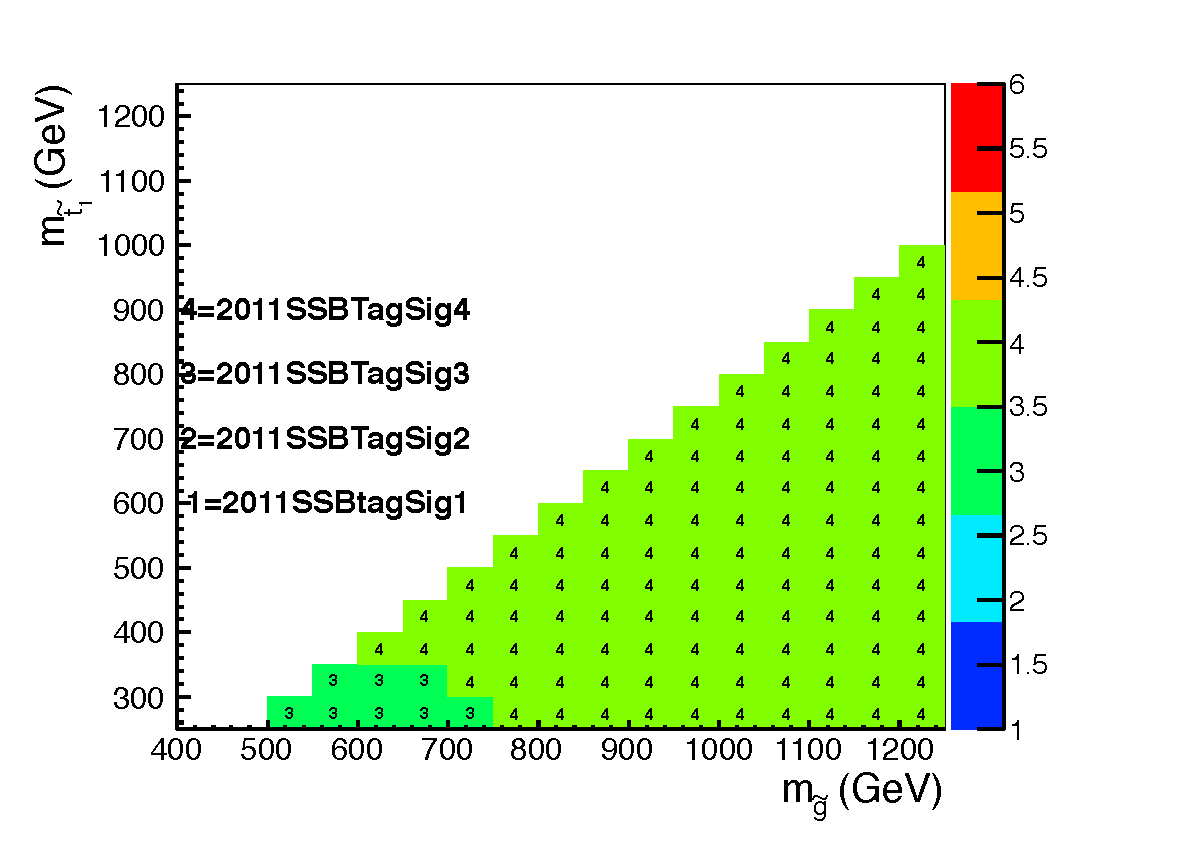
\includegraphics[width=0.65\linewidth]{figs/gluinostopsigreg.pdf}
\caption{The signal region with the best expected limit as a function of 
$m(\widetilde{g}$ vs. $m(\widetilde{t})$ plane for $m(\chi^0_1)$=50 GeV.
The coding is: 1=(200-50), 2=(200-150), 3=(320-50), and 4=(320-120), where
the first (second) number is the $H_T$ (\met) threshold in GeV. The number
of requested btags is 2 or more.
\label{fig:gluinostoptimize}}
\end{center}
\end{figure}


For each point in parameter space we use the signal region that gives
the best expected limit.  
{\bf (Note: so far the region with 3 btags has not been used).}
Limits are calculated using all experimental
uncertainties; the JES and btag uncertainties are calculated point-by-point.
An example of this optimization is shown in Figure~\ref{fig:gluinostoptimize},
where we show the choice of signal region that gives the best expected limit
in the $m(\widetilde{g})$ vs. $m(\widetilde{t})$ plane for the choice
$m(\chi^0_1)$=50 GeV.



%Using $\met > 50$ GeV and $H_T > 200$ GeV, which corresponds 
%to Table~\ref{tab:yield_ht200met50}: 5 events observed and 3.723 $\pm$ 0.787 $\pm$ 1.23 expected from backgrounds,
%we set a limit at 95\% CL of 7.65 events with the  CL$_{\rm S}$ method. The expected limit is 6.13. 

\subsubsection{Limits for the $\widetilde{g} \to t\widetilde{t}$ Model}
\label{sec:firststoplimits}



The limits on the production cross-section in this model in the 
gluino mass vs. stop mass plane for two choices of the 
LSP mass are shown in Figure~\ref{fig:mglinoStop}
Using the 
NLO$+$NLL cross-section for gluino pair production, we also place a limit
on the mass parameters of this model.  We basicaly can exclude 
$m(\widetilde{g})$ up to about 800 GeV for all kinematically allowed
values of the stop mass: 
$m(t)+m(\chi^0_1)~<~m(\widetilde{t})~<~m(\widetilde{g})-m(t)$. 



\begin{figure}[htb]
\begin{center}
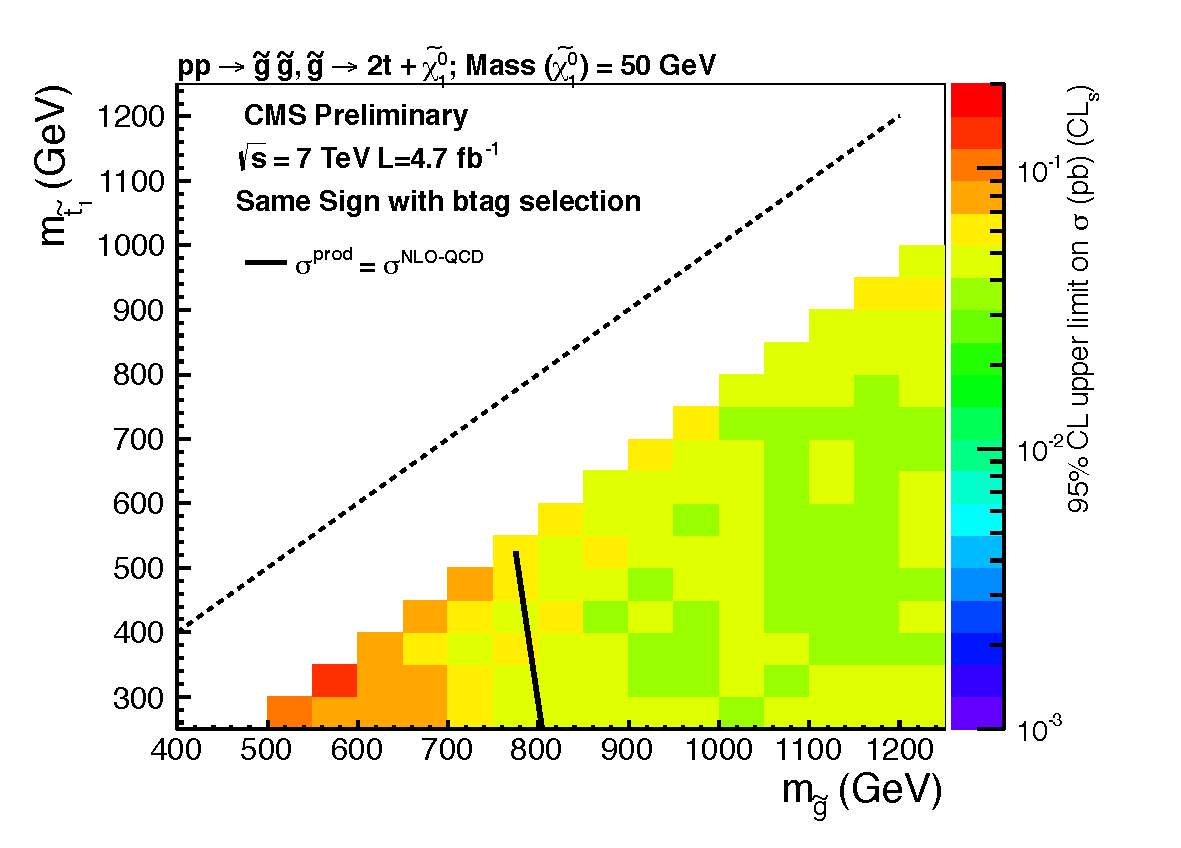
\includegraphics[width=0.47\linewidth]{figs/gluinostop50.pdf}
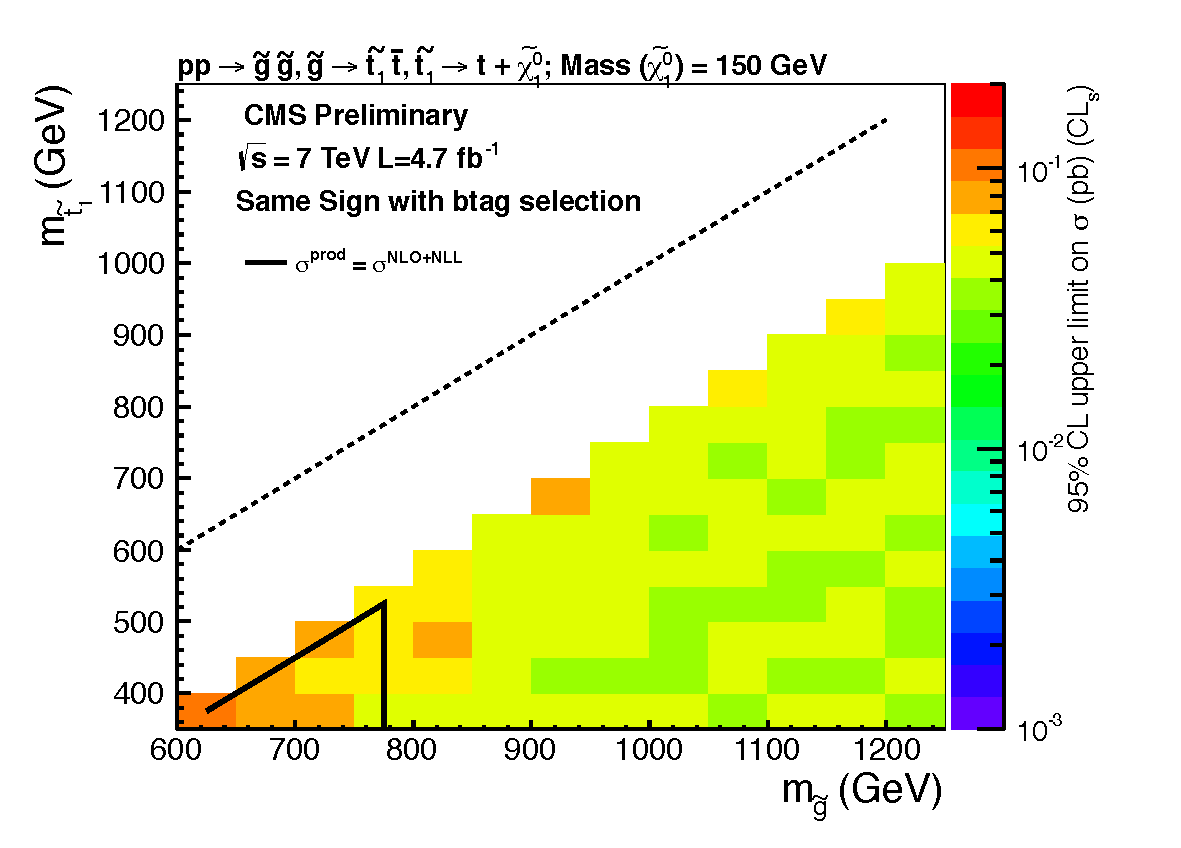
\includegraphics[width=0.47\linewidth]{figs/gluinostop150.pdf}
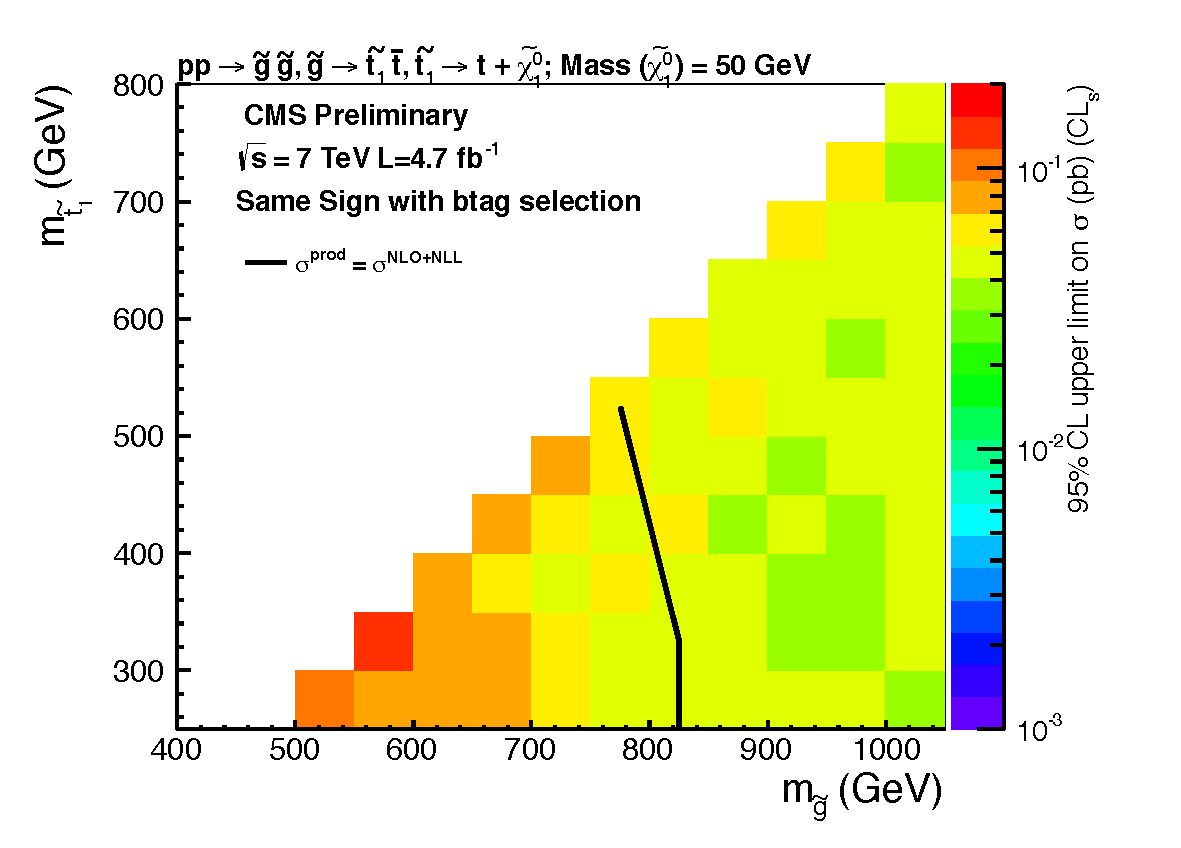
\includegraphics[width=0.47\linewidth]{figs/gluinostop50_zoom.pdf}
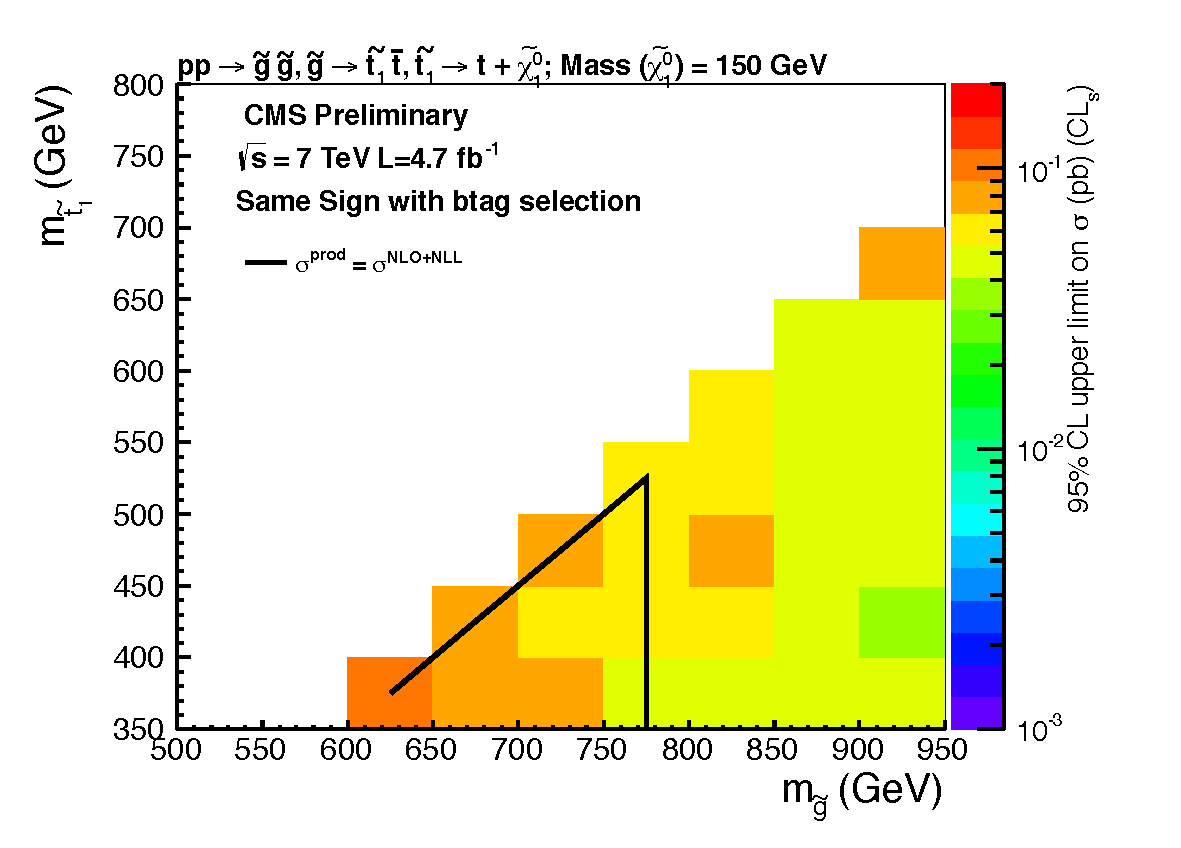
\includegraphics[width=0.47\linewidth]{figs/gluinostop150_zoom.pdf}
\caption{Cross section limits in the $m(\widetilde{g})$ vs. $m(\widetilde{t})$ plane
for $m(\chi_1^0)$ = 50 GeV (left) and 150 GeV (right).  
The bottom plots are versions of the top plots ``zoomed'' into the region
of interest.
\label{fig:mglinoStop}}
\end{center}
\end{figure}


%\subsubsection{What is missing for the $\widetilde{g} \to t\widetilde{t}$ Model}
%\begin{itemize}
%\item Perhaps more details on the MC signal generation???
%\item Need a reference for the {\tt T1tttt} model
%\item Maybe also a plot for LSP mass = 100 GeV? 
%\end{itemize}


\clearpage


\subsection{{\tt T1tttt} Model}
\label{t1ttmodel}

\subsubsection{Theoretical discussion of the {\tt T1tttt} Model}
\label{sec:t1tttheory}
The {\tt T1tttt} simplified model\cite{T1tttt} is very similar to the model of 
Section~\ref{sec:firststopmodel}.  In this model it is assumed that all squarks 
are very heavy, but the stop is somewhat lighter than the other 
quarks\cite{stopVirtual}\cite{stopVirtualPRD}.
Then the gluino would decay as $\widetilde{g} \to t\bar{t}\chi_1^0$ through virtual stops.
Other gluino decay modes would be suppressed because the stop is the lightest squark.
The final state after gluino pair production is $tt\bar{t}\bar{t}\chi_1^0\chi_1^0$,
just as in Section~\ref{sec:firststopmodel}.
The model parameters are $M(\widetilde{g})$ and $M(\chi_1^0)$.



\subsubsection{Signal region definition for the {\tt T1tttt} Model}
\label{sec:t1ttttdefinition}
For each point in parameter space we use the signal region that gives
the best expected limit, see Figure~\ref{fig:t1tttoptimize}.
{\bf (Note: so far the region with 3 btags has not been used).}
The limits include all experimental 
uncertainties.   The JES and btag uncertainties are calculated point-by-point.


\begin{figure}[htb]
\begin{center}
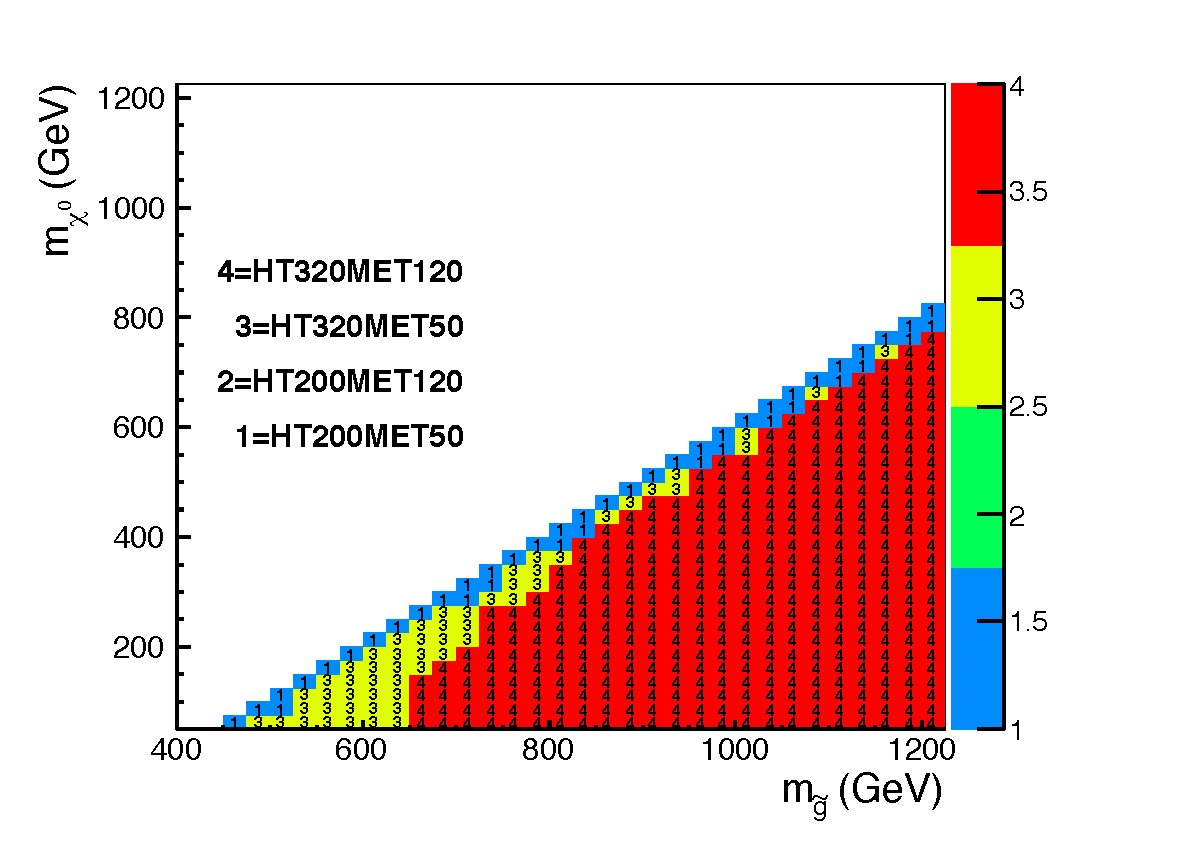
\includegraphics[width=0.4\linewidth]{figs/t1ttttsigreg.pdf}
\caption{The signal region with the best expected limit as a function of 
$m(\widetilde{g})$ vs. $m(\widetilde{t})$ plane for $m(\chi^0_1)$=50 GeV.
The coding is: 1=(200-50), 2=(200-150), 3=(320-50), and 4=(320-120), where
the first (second) number is the $H_T$ (\met) threshold in GeV. The number
of requested btags is 2 or more.
\label{fig:t1tttoptimize}}
\end{center}
\end{figure}


\subsubsection{Limits for the {\tt T1tttt} Model}
\label{sec:t1ttttlimits}
The limit on the production cross-section in this model in the 
gluino mass vs. LSP mass plane shown in Figure~\ref{fig:T1ttttLimit}.  
Using the 
NLO$+$NLL cross-section for gluino pair production, we place a limit
on the mass parameters as shown in Figure~\ref{fig:T1ttttLimit}.
Basically we exclude 
$m(\widetilde{g})$ up to about 800 GeV with a small dependence on 
$m(\chi_1^0)$.

\begin{figure}[htb]
\begin{center}
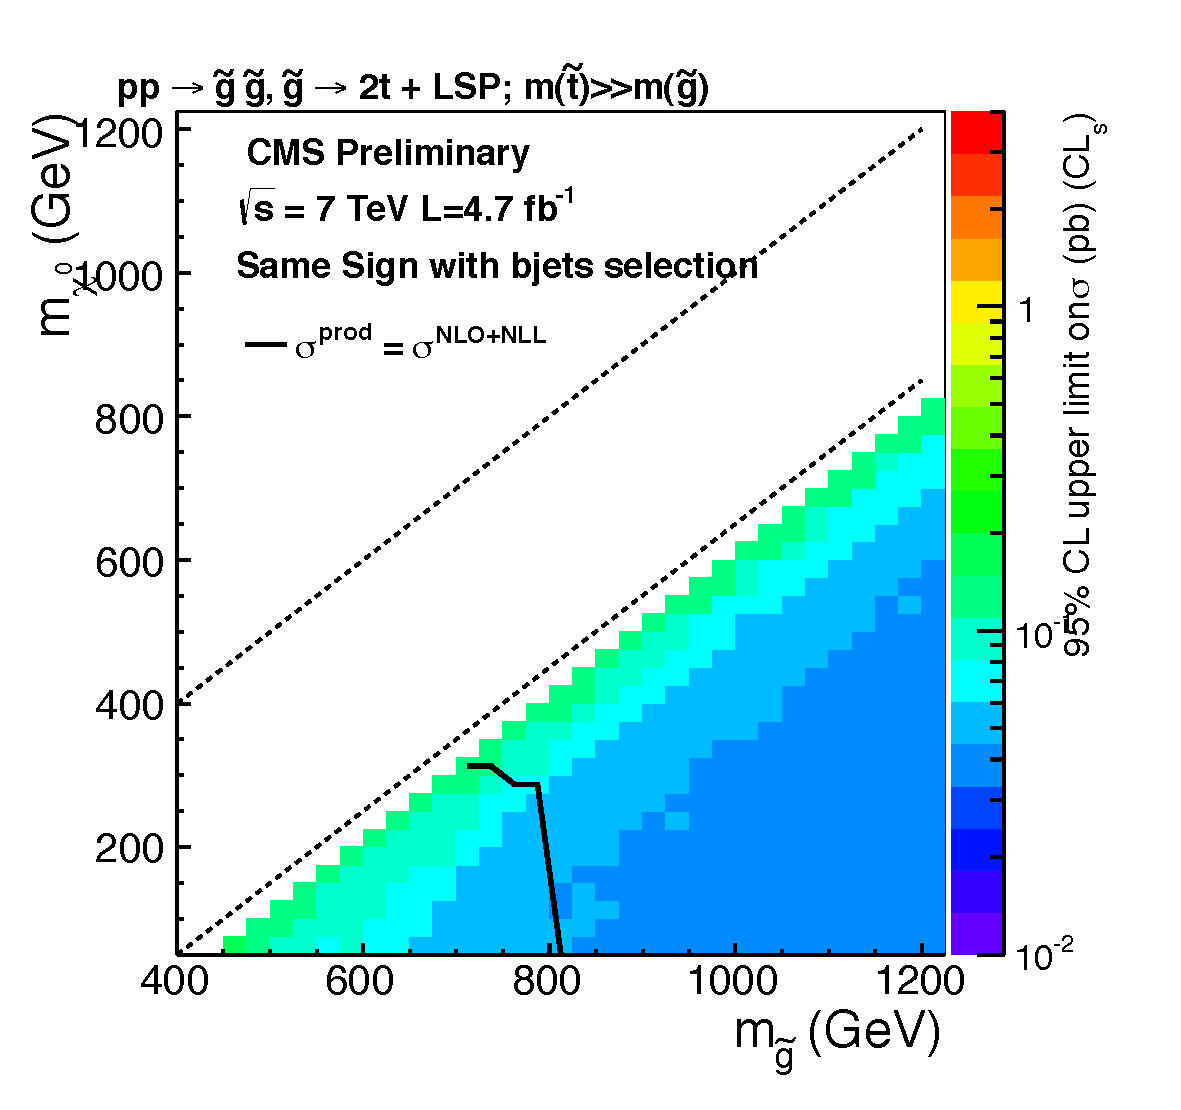
\includegraphics[width=0.48\linewidth]{figs/T1tttt.pdf}
\caption{Cross section limits in the $m(\widetilde{g})$ vs. $m(\chi_1^0)$ plane for the
{\tt T1tttt} model.  
\label{fig:T1ttttLimit}}
\end{center}
\end{figure}

%\subsubsection{What is missing for the {\tt T1tttt} Model}
%\begin{itemize}
%\item Need at least a sentence to say something which signal region contributes.  Or a plot.
%\item Need a reference for the {\tt T1tttt} model
%\end{itemize}


\clearpage

\subsection{Sbottom pair production model}
\label{sec:sbottompair}
In this model we have $pp \to \tilde{b}\tilde{b}$.  The sbottom decays 
as $\tilde{b} \to t\chi^{-}$ followed by $\chi^{-} \to W^- \chi_1^0$. 
The final state is $t\bar{t}W^+W^- \chi_1^0 \chi_1^0$. 
The model parameters are $M(\widetilde{b})$, $M(\chi_1^0)$, and $M(\chi^{\pm})$.
For simplicity we only consider mass parameters such that the $\chi^{-}$ is on shell.

\subsubsection{Signal region definition for the sbottom pair production model}
\label{sec:sbottompairdefinition}
For each point in parameter space we use the signal region that gives
the best expected limit, see Figure~\ref{fig:sbottomoptimize}.
{\bf (Note: so far the region with 3 btags has not been used).}
The limits include all experimental 
uncertainties.   The JES and btag uncertainties are calculated point-by-point.


\begin{figure}[htb]
\begin{center}
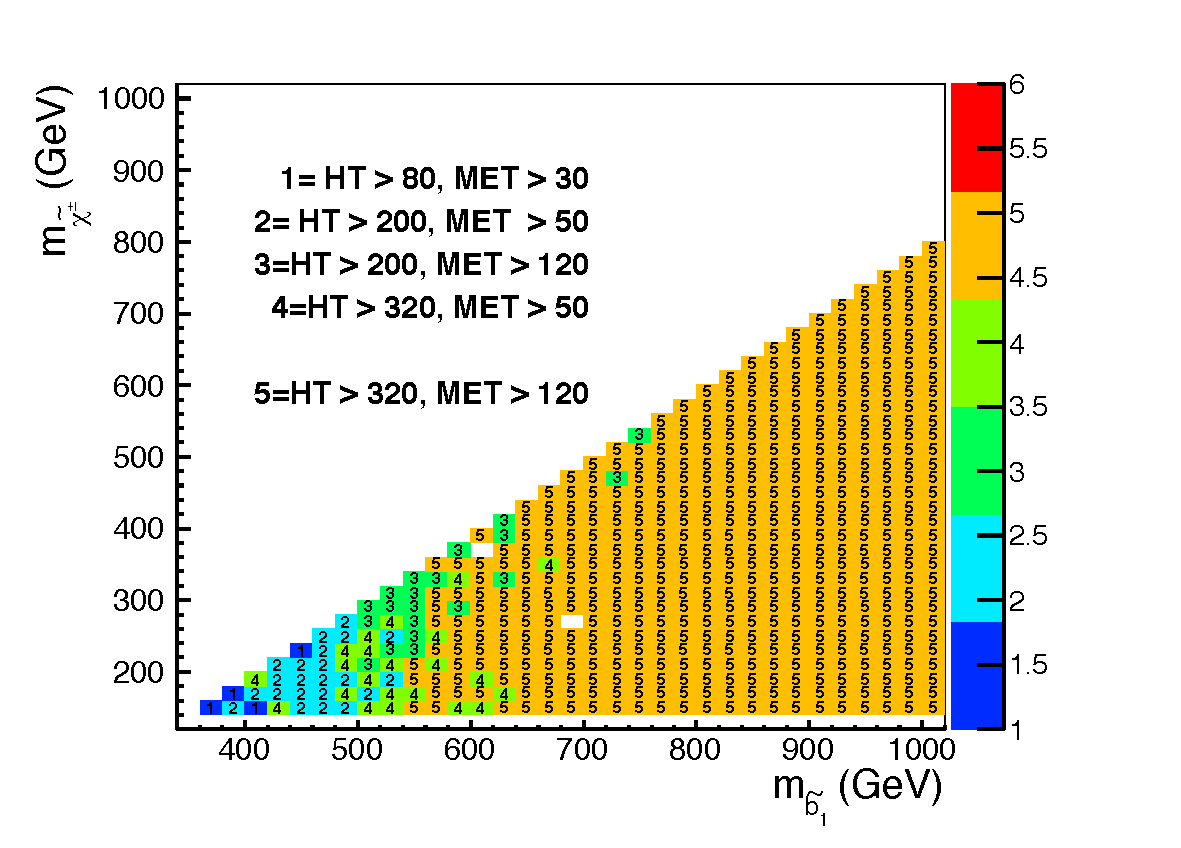
\includegraphics[width=0.5\linewidth]{figs/sbottom_regions.pdf}
\caption{The signal region with the best expected limit as a function of 
$m(\chi^{\pm}))$ vs. $m(\widetilde{b})$ plane for $m(\chi^0_1)$=50 GeV.
The coding is: 1=(80,30),
2=(200-50), 3=(200-150), 4=(320-50), and 5=(320-120), where
the first (second) number is the $H_T$ (\met) threshold in GeV. The number
of requested btags is 2 or more.
\label{fig:sbottomoptimize}}
\end{center}
\end{figure}


\subsubsection{Limits for the sbottom pair production model}
\label{sec:sbottompairlimits}
The limit on the production cross-section in this model in the 
sbottom mass vs. $\chi^{\pm}$ mass plane shown in 
Figure~\ref{fig:sbottomLimit} for 
$m(\chi^0_1)$=50 GeV. 
Using the 
NLO$+$NLL cross-section for gluino pair production, we place a limit
on the mass parameters as shown in Figure~\ref{fig:sbottomLimit}.
We have little sensitivity to the model parameters.
% exclude $m(\widetilde{b})$ up to about 450 GeV for all
% kinematically allowed values of the chargino mass:
% $m(\chi^{\pm})~<~m(\widetilde{b})-m(t)$.

\begin{figure}[htb]
\begin{center}
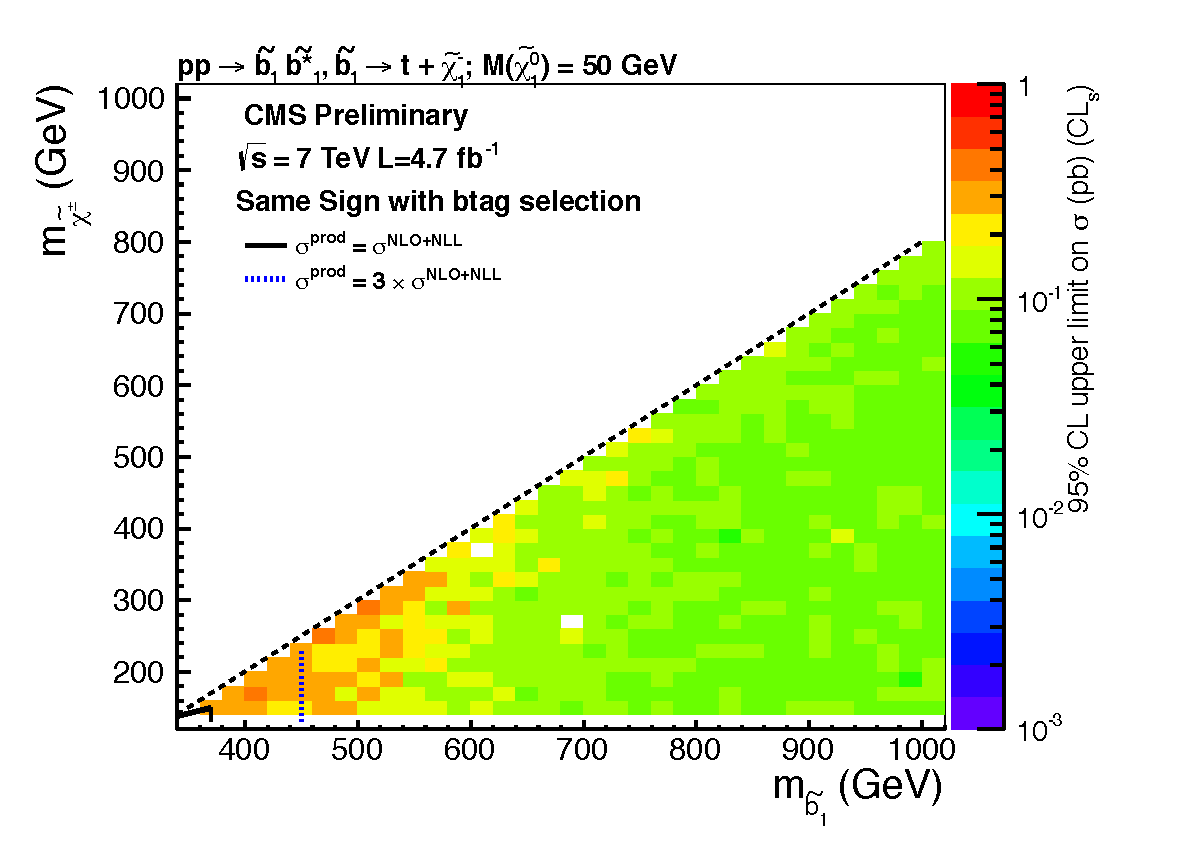
\includegraphics[width=0.48\linewidth]{figs/sbottom_limit.pdf}
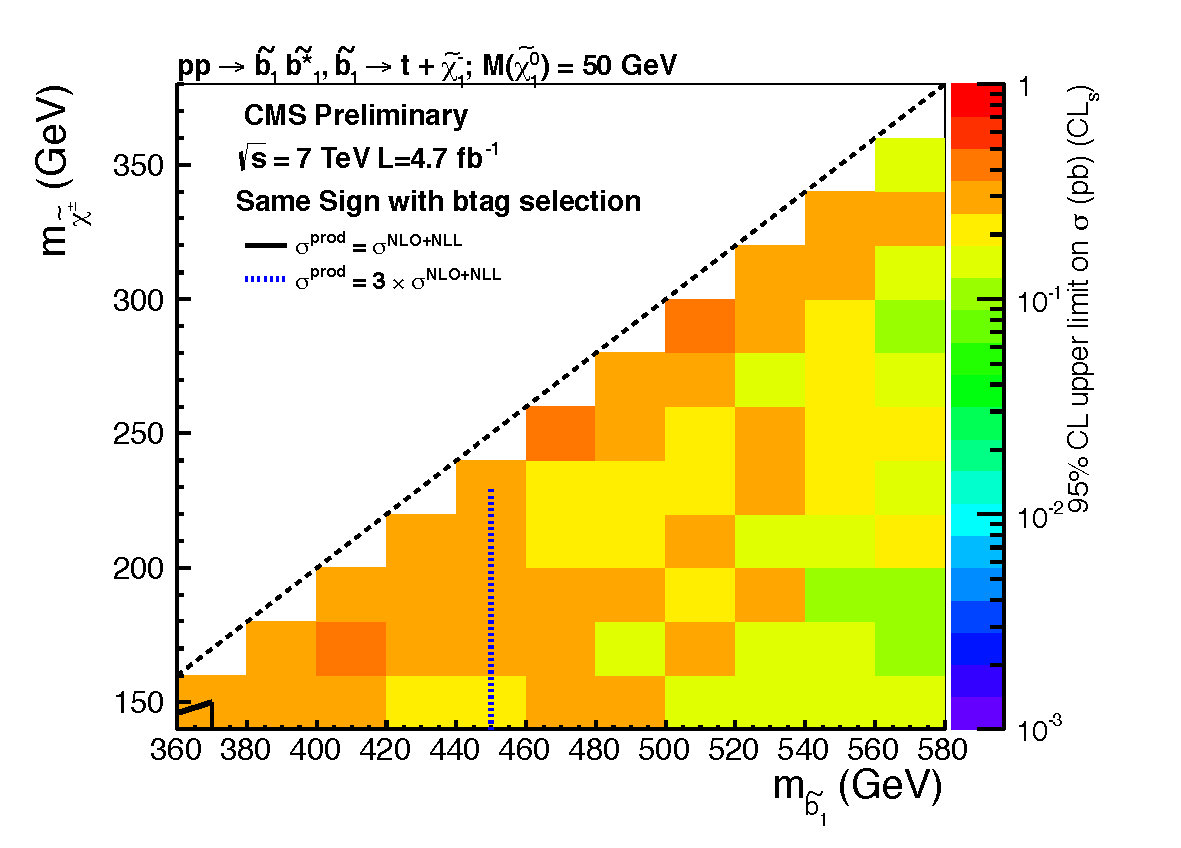
\includegraphics[width=0.48\linewidth]{figs/sbottom_limit_zoom.pdf}
\caption{Cross section limits in the $m(\widetilde{b})$ vs. $m(\chi^{\pm})$ 
plane for the sbottom pair production model with 
$m(\chi^0_1)$=50 GeV.  The rigth plot is a ``zoomed'' in version 
of the left plot.\label{fig:sbottomLimit}}
\end{center}
\end{figure}





%\subsubsection{What is missing for the sbottom pair production model}
%\begin{itemize}
%\item Everything in Sections~\ref{sec:sbottompairdefinition} and \ref{sec:sbottompairlimits}
%\item It would be nice to have a reference.  I am not sure that the references that
%we have on our twiki are appropriate. 
%\item Perhaps more details on the MC signal generation
%\end{itemize}

\clearpage

\subsection{$\widetilde{g} \to \widetilde{b}\bar{b}$ Model}
\label{sec:gbb}
This model is mostly gluino pair production followed by 
$\widetilde{g} \to \widetilde{b}\bar{b}$, $\widetilde{b} \to t \chi^{-}$ and
$\chi^{-} \to W^- \chi_1^0$. 
The final state is $t\bar{t}b\bar{b}W^+W^- \chi_1^0 \chi_1^0$
or $ttb\bar{b}W^+W^- \chi_1^0 \chi_1^0$ $(+ c.c.)$.
The model also includes the $b g \to \widetilde{b} \widetilde{g}$ process,
in which case the final state is
$tb\bar{b}W^+W^- \chi_1^0 \chi_1^0$ $(+ c.c.)$. 
The model parameters are $M(\widetilde{g})$
$M(\widetilde{b})$, $M(\chi_1^0)$, and $M(\chi^{\pm})$.
For simplicity we only consider mass parameters such that the $\chi^{-}$ is on shell.

\subsubsection{Signal region definition for the $\widetilde{g} \to \widetilde{b}\bar{b}$ Model}
\label{sec:gbbdefinition}

\begin{figure}[htb]
\begin{center}
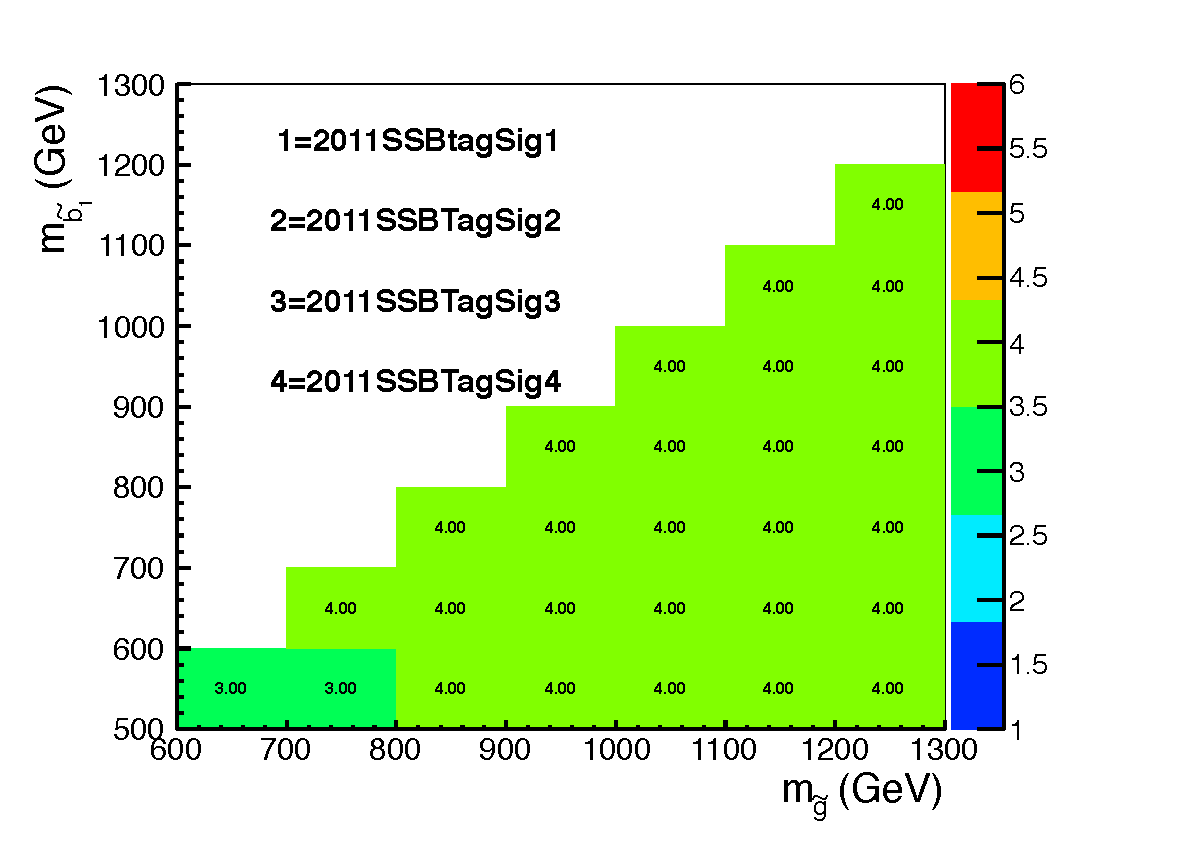
\includegraphics[width=0.65\linewidth]{figs/gl_sb_300_50_regions.pdf}
\caption{The signal region with the best expected limit as a function of 
$m(\widetilde{g}$ vs. $m(\widetilde{b})$ for $m(\chi^0_1)$=50 GeV
and $m(\chi^{\pm})$=200 GeV. 
The coding is: 1=(200-50), 2=(200-150), 3=(320-50), and 4=(320-120), where
the first (second) number is the $H_T$ (\met) threshold in GeV. The number
of requested btags is 2 or more.
\label{fig:gluinosboptimize}}
\end{center}
\end{figure}


For each point in parameter space we use the signal region that gives
the best expected limit.  
{\bf (Note: so far the region with 3 btags has not been used).}
Limits are calculated using all experimental
uncertainties; the JES and btag uncertainties are calculated point-by-point.
An example of this optimization is shown in Figure~\ref{fig:gluinosboptimize},
where we show the choice of signal region that gives the best expected limit
in the $m(\widetilde{g})$ vs. $m(\widetilde{b})$ plane for the choice
$m(\chi^0_1)$=50 GeV and $m(\chi^{\pm})$=200 GeV. 
Roughly speaking we we exclude gluino masses below about 750 GeV for 
all sbottom masses kinematically accessible, {\it i.e.}, 
$m(t)+m(\chi^{\pm})~<~m(\widetilde{b}~<~m(\widetilde{g})$.



\subsubsection{Limits for the $\widetilde{g} \to \widetilde{b}\bar{b}$ Model}
\label{sec:gbblimits}

The limits on the production cross-section in this model in the 
gluino mass vs. sbottom mass plane for two choices of the 
chargino mass and an LSP mass of 50 GeV 
are shown in Figure~\ref{fig:mglinoSbottom}
Using the 
NLO$+$NLL cross-section for gluino pair production, we also place a limit
on the mass parameters of this model.


\begin{figure}[htb]
\begin{center}
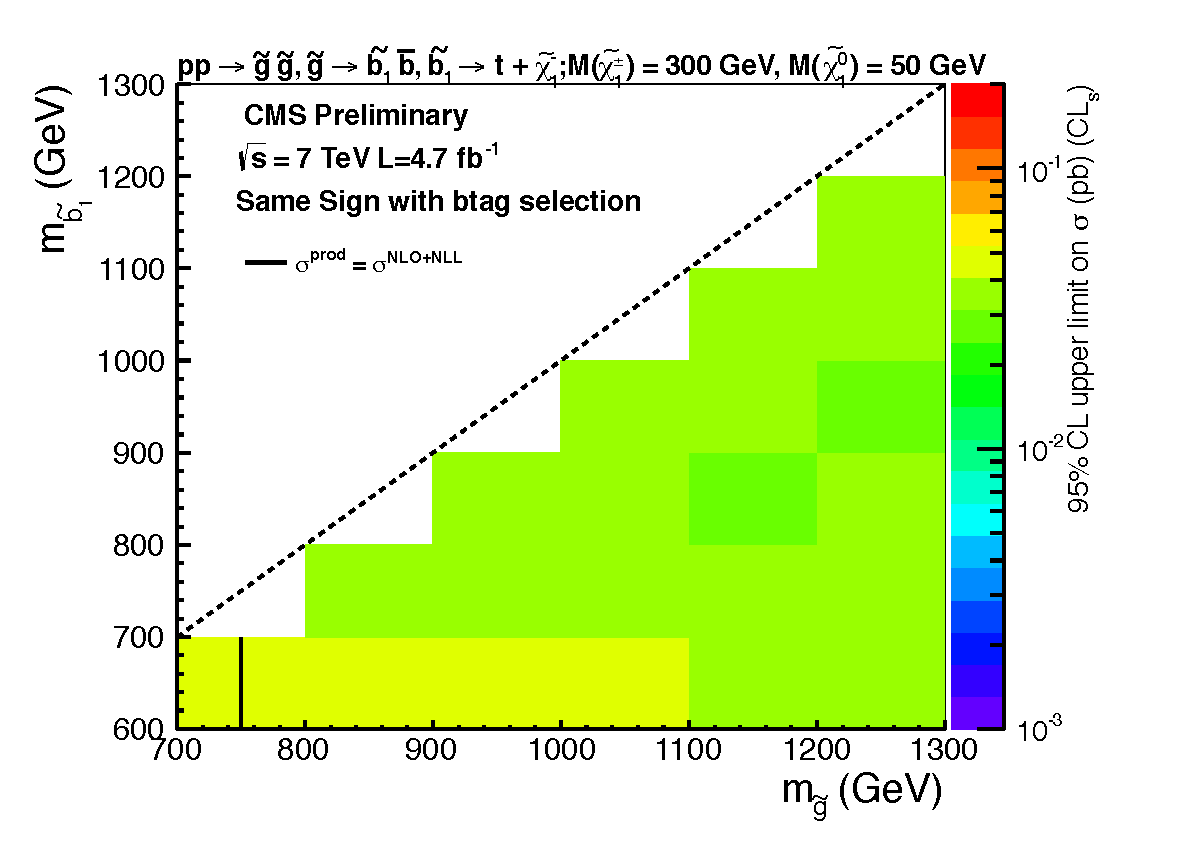
\includegraphics[width=0.47\linewidth]{figs/gl_sb_300_50.pdf}
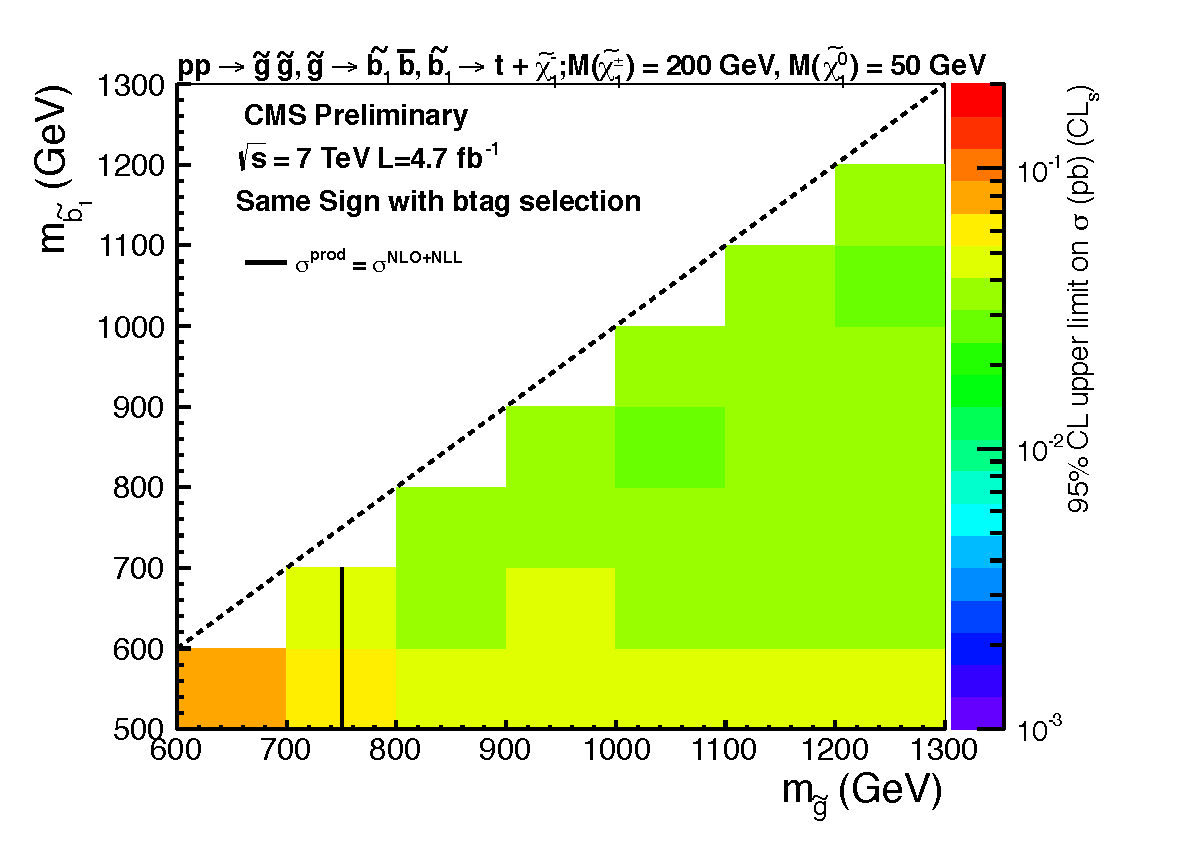
\includegraphics[width=0.47\linewidth]{figs/gl_sb_200_50.pdf}
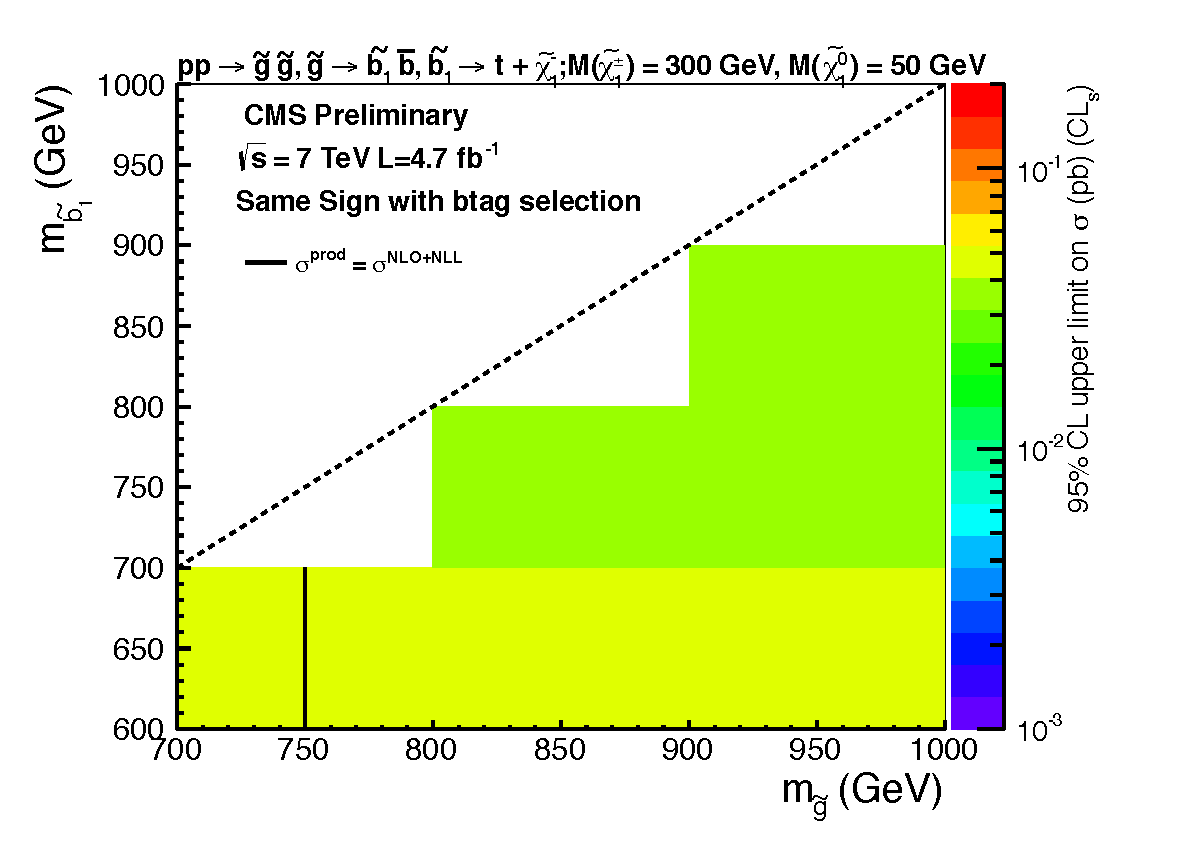
\includegraphics[width=0.47\linewidth]{figs/gl_sb_300_50_zoom.pdf}
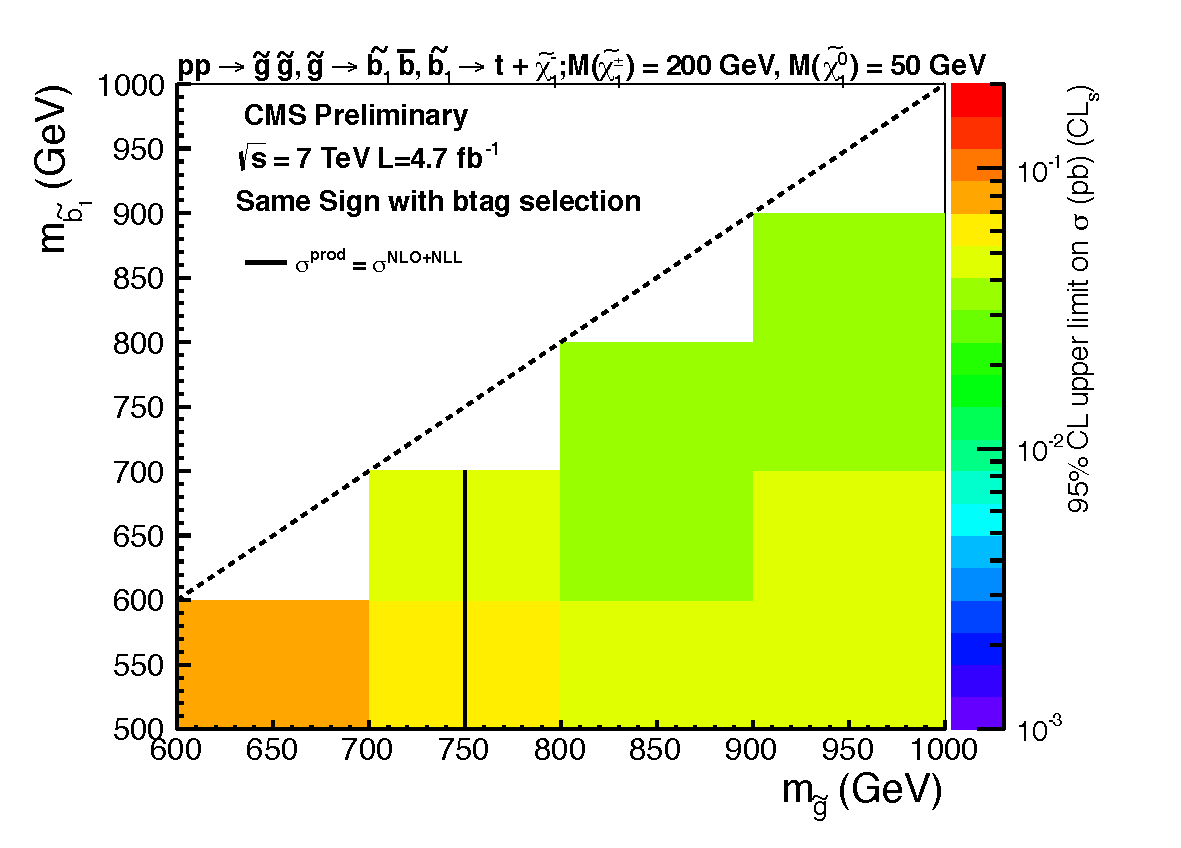
\includegraphics[width=0.47\linewidth]{figs/gl_sb_200_50_zoom.pdf}
\caption{Cross section limits in the $m(\widetilde{g})$ vs. 
$m(\widetilde{b})$ plane
for $m(\chi_1^0)$ = 50 GeV and 
$m(\chi^{\pm})$ = 300 GeV (left) and 200 GeV (right). 
The bottom plots are ``zoomed'' in versions of the top plots.
\label{fig:mglinoSbottom}}
\end{center}
\end{figure}

%\subsubsection{What is missing for the $\widetilde{g} \to \widetilde{b}\bar{b}$ Model}
%\begin{itemize}
%\item Everything in Sections~\ref{sec:gbbdefinition} and \ref{sec:gbblimits}
%\item It would be nice to have a reference.  I am not sure that the 
%references that
%we have on our twiki are appropriate. 
%\item Perhaps more details on the MC signal generation
%\end{itemize}

\clearpage

\section{Conclusion}
\label{sec:conclusion}

We have assessed the sensitivity to mSUGRA of a generic signal characterized by two isolated, high $p_T$ leptons,
significant jet activity, and \met. We performed a scan of the mSUGRA $m_{0}-m_{1/2}$ parameter space and determined  
the expected excluded region in the case of no observed signal as well as the $5\sigma$ sensitivity reach for both SS
and OS dileptons, assuming integrated luminosities of 100 pb$^{-1}$ and 1 fb$^{-1}$. Our results indicate that we are sensitive to a
significant region of the mSUGRA parameter space which extends upon previous results from the Tevatron. 




\clearpage
\begin{thebibliography}{99}

\bibitem{cdf:recentSusy} {CDF Trilepton Search, 2009, CDF/PUB/EXOTIC/PUBLIC/9817};\\
{\small \tt http://www-cdf.fnal.gov/physics/exotic/r2a/20090521.trilepton\_3fb/Welcome.html}
%\bibitem{cdf:recentSusy1} {``Inclusive Search for Squark and Gluino Production in $p\bar{p}$ Collisions at $\sqrt{s}$ = 1.96-TeV'', Phys.Rev.Lett.102:121801, (2009).}
\bibitem{d0:recentSusy} {``Search for associated production of charginos and neutralinos in the trilepton final state using 2.3 fb$^{-1}$ of data'', Phys. Lett. B 680, 34 (2009).}
%\bibitem{d0:recentSusy1} {``Search for squarks and gluinos in events with jets and missing transverse energy using 2.1 fb$^{-1}$ of ppbar collision data at $sqrt(s)=1.96$ TeV'', 
%Phys. Lett. B 660 , 449 (2008).}

\bibitem{osnote} {``Data driven background estimate for a new physics search with opposite sign dileptons''}, CMS AN-2009/130.

\bibitem{ssnote} {``Data driven background study for new physics searches with same sign dileptons at $\sqrt{s} = 10 $ TeV''}, CMS AN-2009/138.

\bibitem{mcsusy}{\tt https://twiki.cern.ch/twiki/bin/viewauth/CMS/SUSYMCRequirements0911}.

\bibitem{fast10}{\tt https://twiki.cern.ch/twiki/bin/view/CMS/SUSY33XScan}.

\bibitem{ww} {``Prospects for measuring the $WW$ production cross section in $pp$ collisions at $\sqrt s = $10 TeV''}, CMS AN-2009/042 and PAS EWK-09-002.

\bibitem{ttbar} {``Expectations for observation of top quark pair production in the dilepton final state with the early CMS data''}, CMS AN-2009/050 and PAS TOP-09-002.

\bibitem{tcmet} {``Correcting Missing Transverse Energy Using Tracks``} CMS AN-2009/022.

\bibitem{conversionnote} {``Study of photon conversion rejection at CMS''}, CMS AN-2009/159.

\bibitem{glbtrk} {\tt https://hypernews.cern.ch/HyperNews/CMS/get/muon/258.html}.

\bibitem{muonid} {``Muon Identification in CMS''}, CMS AN-2008/098.

\bibitem{vplusj} {\tt https://twiki.cern.ch/twiki/bin/view/CMS/VplusJets}.

\bibitem{fakenote} {``Data-driven methods to estimate the electron and muon fake contributions to lepton analyses''}, CMS AN-2009/041.

\bibitem{cite:cousins} {``Evaluation of three methods for calculating statistical significance when incorporating a systematic uncertainty into a test of the background-only hypothesis for a Poisson process''} arXiv:physics/0702156 [physics.data-an]

\bibitem{cite:conway} {``Interval estimation in the presence of nuisance parameters. 1. Bayesian approach''} arXiv:physics/0409129v1 [physics.data-an]

\bibitem{lep:lepsusyreach}{LEP Susy working group: {\tt http://lepsusy.web.cern.ch/lepsusy/} }

\bibitem{bayes}{\tt http://arxiv.org/pdf/physics/0409129}

\bibitem{victor} {\tt http://arxiv.org/pdf/0906.5016}; \\
{\tt http://indico.cern.ch/contributionDisplay.py?contribId=2\&confId=39042}.

\bibitem{summer09}{\tt https://twiki.cern.ch/twiki/bin/view/CMS/SUSY31XProduction}.


\end{thebibliography}

\end{document}
